
\section{Strategies for model evaluation}

\begin{frame}{Model evaluation: Rationale}
    \only<1>{
        \textbf{\underline{Statistical inference:}}\\
        Goal: In-sample quantification
        \vspace{0.7cm}\\
        \textbf{\underline{Predictive modelling:}}\\
        Goal: Out-of-sample generalization
    }
    \only<2>{
        \centering
        How can we test how good our model is on \textbf{unseen data} and \textbf{be certain that this predictive performance holds if we present even more new data}
    }
\end{frame}


\begin{frame}{Model evaluation: Validation set} % Performance
    \centering
    \begin{tikzpicture}
        \node[] at (-4, 1) {};
        \node[] at (4, -4.5) {};
        \visible<1-5>{
            \node[minimum height=0.5cm, minimum width=7.5cm, draw=black, fill=gray!20, label=\small{Dataset}] (full) at (0, 0) {};
        }

        \visible<2-5,7-9>{
            \node[minimum height=0.5cm, minimum width=6cm, draw=black, fill=green!20, anchor=west, label=below:\footnotesize{Training}] (train) at (full.west) {};
            \node[minimum height=0.5cm, minimum width=1.5cm, draw=black, fill=blue!20, anchor=east, label=below:\footnotesize{Validation}] (val) at (full.east) {};
        }

        \visible<3-5,7-9>{
            \node[draw=black, dashed, align=center, font=\small\linespread{0.9}\selectfont] (model) at ($ (train) - (0, 2.5) $) {Model\\fitting};
            \draw[->] ($ (train.south) - (0, 0.5) $) -- (model.north);
        }

        \visible<4-5,7-9>{
            \node[draw=black, dashed, align=center, font=\small\linespread{0.9}\selectfont] (eval) at ($ (val) - (0, 2.5) $) {Evaluation};
            \draw[->] ($ (val.south) - (0, 0.5) $) -- (eval.north);
            \draw[->] (model.east) -- (eval.west) node [midway, above, sloped] {\scriptsize{Model}};
        }

        \visible<5,7-9>{
            \node[align=center, font=\small\linespread{0.9}\selectfont] (score) at ($ (eval) - (0, 1.5) $) {Predictive\\performance};
            \draw[->] ($ (eval.south) - (0, 00) $) -- (score.north);
        }
        \visible<6>{
            \node[text width=11cm] at (0, -1.75) {
                In the validation set approach we split the dataset into two subsets (commonly $\sim$80\%/20\%), use the first for training the model and the second to test its performance.
                \begin{itemize}
                    \item[\textcolor{green}{+}] Accurate estimate of out-of-sample error
                    \item[\textcolor{green}{+}] Simple
                    \item[\textcolor{red}{-}] Variable results depending on the exact split
                    \item[\textcolor{red}{-}] Only uses a subset of data for training models
                    \item[\textcolor{red}{-}] Gives a point estimate of the error, without confidence intervals
                \end{itemize}
            };
        }
        \visible<7-9>{
            \node[align=center, font=\small\linespread{0.9}\selectfont] (trainscore) at ($ (model) - (0, 1.5) $) {Training\\performance};
            \draw[->] ($ (model.south) - (0, 00) $) -- (trainscore.north);
        }
        \visible<8-9>{
            \node[] at ($ (trainscore.east)!0.5!(score.west) $) {\textcolor{red}{$\neq$}};
        }
        \visible<9>{
            \node[align=center, font=\small\linespread{0.9}\selectfont] (traincharacteristics) at ($ (train) + (0, 1) $) {Males\\>60 years};
            \node[align=center, font=\small\linespread{0.9}\selectfont] (valcharacteristics) at ($ (val) + (0, 1) $) {Females\\<40 years};

            \draw[->, densely dotted] (traincharacteristics.south) -- ($ (traincharacteristics.south) - (0, 0.3) $);
            \draw[->, densely dotted] (valcharacteristics.south) -- ($ (valcharacteristics.south) - (0, 0.3) $);
        }

    \end{tikzpicture}
\end{frame}

\begin{frame}{Model evaluation: Stratification} % Definition
    \textbf{\underline{Stratification:}}\\
    Ensuring all folds of the dataset are similar with respect to some given characteristics.
\end{frame}

\begin{frame}{Model evaluation: Stratification} % Dataset
    \only<1-6>{
        \centering
        \begin{tikzpicture}
            \node[] at (-5, 1) {};
            \node[] at (5, -6) {};

            \node[minimum height=0.5cm, minimum width=7.5cm, draw=black, fill=gray!20, label=\small{Dataset}] (full) at (0, 0) {};

            \visible<1-2>{
                \PythonInputNode{1}{(-3.5, -2.5)}{pythonnode}{7cm}{8}{
                    df = ...^^J
                    ^^J
                    ^^J
                    ^^J
                    ^^J
                    ^^J
                }
            }
            \visible<2-3>{
                \node[minimum height=0.5cm, minimum width=0.375cm, draw=black, fill=red!40, anchor=west, inner sep=0pt, outer sep=0pt] (p1) at (full.west) {};
                \node[minimum height=0.5cm, minimum width=0.375cm, draw=black, fill=blue!70, anchor=west, inner sep=0pt, outer sep=0pt] (p2) at (p1.east) {};
                \node[minimum height=0.5cm, minimum width=0.375cm, draw=black, fill=blue!50, anchor=west, inner sep=0pt, outer sep=0pt] (p3) at (p2.east) {};
                \node[minimum height=0.5cm, minimum width=0.375cm, draw=black, fill=blue!30, anchor=west, inner sep=0pt, outer sep=0pt] (p4) at (p3.east) {};
                \node[minimum height=0.5cm, minimum width=0.375cm, draw=black, fill=red!80, anchor=west, inner sep=0pt, outer sep=0pt] (p5) at (p4.east) {};
                \node[minimum height=0.5cm, minimum width=0.375cm, draw=black, fill=blue!80, anchor=west, inner sep=0pt, outer sep=0pt] (p6) at (p5.east) {};
                \node[minimum height=0.5cm, minimum width=0.375cm, draw=black, fill=blue!20, anchor=west, inner sep=0pt, outer sep=0pt] (p7) at (p6.east) {};
                \node[minimum height=0.5cm, minimum width=0.375cm, draw=black, fill=red!90, anchor=west, inner sep=0pt, outer sep=0pt] (p8) at (p7.east) {};
                \node[minimum height=0.5cm, minimum width=0.375cm, draw=black, fill=blue!75, anchor=west, inner sep=0pt, outer sep=0pt] (p9) at (p8.east) {};
                \node[minimum height=0.5cm, minimum width=0.375cm, draw=black, fill=blue!85, anchor=west, inner sep=0pt, outer sep=0pt] (p10) at (p9.east) {};
                \node[minimum height=0.5cm, minimum width=0.375cm, draw=black, fill=blue!75, anchor=west, inner sep=0pt, outer sep=0pt] (p11) at (p10.east) {};
                \node[minimum height=0.5cm, minimum width=0.375cm, draw=black, fill=red!50, anchor=west, inner sep=0pt, outer sep=0pt] (p12) at (p11.east) {};
                \node[minimum height=0.5cm, minimum width=0.375cm, draw=black, fill=red!65, anchor=west, inner sep=0pt, outer sep=0pt] (p13) at (p12.east) {};
                \node[minimum height=0.5cm, minimum width=0.375cm, draw=black, fill=blue!45, anchor=west, inner sep=0pt, outer sep=0pt] (p14) at (p13.east) {};
                \node[minimum height=0.5cm, minimum width=0.375cm, draw=black, fill=red!45, anchor=west, inner sep=0pt, outer sep=0pt] (p15) at (p14.east) {};
                \node[minimum height=0.5cm, minimum width=0.375cm, draw=black, fill=blue!95, anchor=west, inner sep=0pt, outer sep=0pt] (p16) at (p15.east) {};
                \node[minimum height=0.5cm, minimum width=0.375cm, draw=black, fill=red!25, anchor=west, inner sep=0pt, outer sep=0pt] (p17) at (p16.east) {};
                \node[minimum height=0.5cm, minimum width=0.375cm, draw=black, fill=red!40, anchor=west, inner sep=0pt, outer sep=0pt] (p18) at (p17.east) {};
                \node[minimum height=0.5cm, minimum width=0.375cm, draw=black, fill=red!45, anchor=west, inner sep=0pt, outer sep=0pt] (p19) at (p18.east) {};
                \node[minimum height=0.5cm, minimum width=0.375cm, draw=black, fill=red!15, anchor=west, inner sep=0pt, outer sep=0pt] (p20) at (p19.east) {};
            }
            \visible<2-4>{
                \node[draw=black, fill=blue!50] (malelabel) at ($ (full.east) - (2.3, 1) $) {};
                \node[anchor=west] at (malelabel.east) {\footnotesize{Male}};
                \node[anchor=north, draw=black, fill=red!50] (femalelabel) at ($ (malelabel.south) - (0, 0.1) $) {};
                \node[anchor=west] at (femalelabel.east) {\footnotesize{Female}};

                \node[anchor=north, draw=black, shading=vertical, top color=black, bottom color=white, minimum height=0.5825cm] (agelabel) at ($ (malelabel.north) + (1.5, 0) $) {};
                \node[anchor=west] at (agelabel.east) {\footnotesize{Age}};
            }
            \visible<3>{
                \PythonInputNode{1}{(-3.5, -2.5)}{pythonnode}{7cm}{8}{
                    df = ...^^J
                    ^^J
                    train = df.iloc[:int(len(df) * 0.8)]^^J
                    validation = df.iloc[int(len(df) * 0.8):]^^J
                    ^^J
                    ^^J
                }
            }
            \visible<3,6>{
                \node[minimum height=0.5cm, minimum width=6cm, draw=none, fill=none, anchor=west, label=below:\footnotesize{Training}] (train) at (full.west) {};
                \node[minimum height=0.5cm, minimum width=1.5cm, draw=none, fill=none, anchor=east, label=below:\footnotesize{Validation}] (val) at (full.east) {};
            }
            \visible<4>{
                \PythonInputNode{1}{(-3.5, -2.5)}{pythonnode}{7cm}{8}{
                    df = ...^^J
                    df = df.sort_values(['sex', 'age'])^^J
                    ^^J
                    ^^J
                    ^^J
                    ^^J
                }
            }
            \visible<4-5>{
                \node[minimum height=0.5cm, minimum width=0.375cm, draw=black, fill=red!15, anchor=west, inner sep=0pt, outer sep=0pt] (p1) at (full.west) {};
                \node[minimum height=0.5cm, minimum width=0.375cm, draw=black, fill=blue!20, anchor=west, inner sep=0pt, outer sep=0pt] (p2) at (p1.east) {};
                \node[minimum height=0.5cm, minimum width=0.375cm, draw=black, fill=red!25, anchor=west, inner sep=0pt, outer sep=0pt] (p3) at (p2.east) {};
                \node[minimum height=0.5cm, minimum width=0.375cm, draw=black, fill=blue!30, anchor=west, inner sep=0pt, outer sep=0pt] (p4) at (p3.east) {};
                \node[minimum height=0.5cm, minimum width=0.375cm, draw=black, fill=red!40, anchor=west, inner sep=0pt, outer sep=0pt] (p5) at (p4.east) {};
                \node[minimum height=0.5cm, minimum width=0.375cm, draw=black, fill=blue!45, anchor=west, inner sep=0pt, outer sep=0pt] (p6) at (p5.east) {};
                \node[minimum height=0.5cm, minimum width=0.375cm, draw=black, fill=red!40, anchor=west, inner sep=0pt, outer sep=0pt] (p7) at (p6.east) {};
                \node[minimum height=0.5cm, minimum width=0.375cm, draw=black, fill=blue!50, anchor=west, inner sep=0pt, outer sep=0pt] (p8) at (p7.east) {};
                \node[minimum height=0.5cm, minimum width=0.375cm, draw=black, fill=red!45, anchor=west, inner sep=0pt, outer sep=0pt] (p9) at (p8.east) {};
                \node[minimum height=0.5cm, minimum width=0.375cm, draw=black, fill=blue!70, anchor=west, inner sep=0pt, outer sep=0pt] (p10) at (p9.east) {};
                \node[minimum height=0.5cm, minimum width=0.375cm, draw=black, fill=red!45, anchor=west, inner sep=0pt, outer sep=0pt] (p11) at (p10.east) {};
                \node[minimum height=0.5cm, minimum width=0.375cm, draw=black, fill=blue!75, anchor=west, inner sep=0pt, outer sep=0pt] (p12) at (p11.east) {};
                \node[minimum height=0.5cm, minimum width=0.375cm, draw=black, fill=red!50, anchor=west, inner sep=0pt, outer sep=0pt] (p13) at (p12.east) {};
                \node[minimum height=0.5cm, minimum width=0.375cm, draw=black, fill=blue!75, anchor=west, inner sep=0pt, outer sep=0pt] (p14) at (p13.east) {};
                \node[minimum height=0.5cm, minimum width=0.375cm, draw=black, fill=red!65, anchor=west, inner sep=0pt, outer sep=0pt] (p15) at (p14.east) {};
                \node[minimum height=0.5cm, minimum width=0.375cm, draw=black, fill=blue!80, anchor=west, inner sep=0pt, outer sep=0pt] (p16) at (p15.east) {};
                \node[minimum height=0.5cm, minimum width=0.375cm, draw=black, fill=red!80, anchor=west, inner sep=0pt, outer sep=0pt] (p17) at (p16.east) {};
                \node[minimum height=0.5cm, minimum width=0.375cm, draw=black, fill=blue!85, anchor=west, inner sep=0pt, outer sep=0pt] (p18) at (p17.east) {};
                \node[minimum height=0.5cm, minimum width=0.375cm, draw=black, fill=red!90, anchor=west, inner sep=0pt, outer sep=0pt] (p19) at (p18.east) {};
                \node[minimum height=0.5cm, minimum width=0.375cm, draw=black, fill=blue!95, anchor=west, inner sep=0pt, outer sep=0pt] (p20) at (p19.east) {};
            }
            \visible<5>{
                \draw[->, red] ($ (p1.north) + (0, 0.5) $) -- (p1);
                \draw[->, red] ($ (p6.north) + (0, 0.5) $) -- (p6);
                \draw[->, red] ($ (p11.north) + (0, 0.5) $) -- (p11);
                \draw[->, red] ($ (p16.north) + (0, 0.5) $) -- (p16);
            }
            \visible<5-6>{
                \PythonInputNode{1}{(-3.5, -2.5)}{pythonnode}{7cm}{8}{
                    df = ...^^J
                    df = df.sort_values(['sex', 'age'])^^J
                    ^^J
                    df['fold'] = np.arange(len(df)) \% (1 / 0.2)^^J
                    train = df[df['fold'] != 0]^^J
                    val = df[df['fold'] == 0]^^J
                }
            }
            \visible<6>{
                \node[minimum height=0.5cm, minimum width=0.375cm, draw=black, fill=blue!20, anchor=west, inner sep=0pt, outer sep=0pt] (p1) at (full.west) {};
                \node[minimum height=0.5cm, minimum width=0.375cm, draw=black, fill=red!25, anchor=west, inner sep=0pt, outer sep=0pt] (p2) at (p1.east) {};
                \node[minimum height=0.5cm, minimum width=0.375cm, draw=black, fill=blue!30, anchor=west, inner sep=0pt, outer sep=0pt] (p3) at (p2.east) {};
                \node[minimum height=0.5cm, minimum width=0.375cm, draw=black, fill=red!40, anchor=west, inner sep=0pt, outer sep=0pt] (p4) at (p3.east) {};
                \node[minimum height=0.5cm, minimum width=0.375cm, draw=black, fill=red!40, anchor=west, inner sep=0pt, outer sep=0pt] (p5) at (p4.east) {};
                \node[minimum height=0.5cm, minimum width=0.375cm, draw=black, fill=blue!50, anchor=west, inner sep=0pt, outer sep=0pt] (p6) at (p5.east) {};
                \node[minimum height=0.5cm, minimum width=0.375cm, draw=black, fill=red!45, anchor=west, inner sep=0pt, outer sep=0pt] (p7) at (p6.east) {};
                \node[minimum height=0.5cm, minimum width=0.375cm, draw=black, fill=blue!70, anchor=west, inner sep=0pt, outer sep=0pt] (p8) at (p7.east) {};
                \node[minimum height=0.5cm, minimum width=0.375cm, draw=black, fill=blue!75, anchor=west, inner sep=0pt, outer sep=0pt] (p9) at (p8.east) {};
                \node[minimum height=0.5cm, minimum width=0.375cm, draw=black, fill=red!50, anchor=west, inner sep=0pt, outer sep=0pt] (p10) at (p9.east) {};
                \node[minimum height=0.5cm, minimum width=0.375cm, draw=black, fill=blue!75, anchor=west, inner sep=0pt, outer sep=0pt] (p11) at (p10.east) {};
                \node[minimum height=0.5cm, minimum width=0.375cm, draw=black, fill=red!65, anchor=west, inner sep=0pt, outer sep=0pt] (p12) at (p11.east) {};
                \node[minimum height=0.5cm, minimum width=0.375cm, draw=black, fill=red!80, anchor=west, inner sep=0pt, outer sep=0pt] (p13) at (p12.east) {};
                \node[minimum height=0.5cm, minimum width=0.375cm, draw=black, fill=blue!85, anchor=west, inner sep=0pt, outer sep=0pt] (p14) at (p13.east) {};
                \node[minimum height=0.5cm, minimum width=0.375cm, draw=black, fill=red!90, anchor=west, inner sep=0pt, outer sep=0pt] (p15) at (p14.east) {};
                \node[minimum height=0.5cm, minimum width=0.375cm, draw=black, fill=blue!95, anchor=west, inner sep=0pt, outer sep=0pt] (p16) at (p15.east) {};
                \node[minimum height=0.5cm, minimum width=0.375cm, draw=black, fill=red!15, anchor=west, inner sep=0pt, outer sep=0pt] (p17) at (p16.east) {};
                \node[minimum height=0.5cm, minimum width=0.375cm, draw=black, fill=blue!45, anchor=west, inner sep=0pt, outer sep=0pt] (p18) at (p17.east) {};
                \node[minimum height=0.5cm, minimum width=0.375cm, draw=black, fill=red!45, anchor=west, inner sep=0pt, outer sep=0pt] (p19) at (p18.east) {};
                \node[minimum height=0.5cm, minimum width=0.375cm, draw=black, fill=blue!80, anchor=west, inner sep=0pt, outer sep=0pt] (p20) at (p19.east) {};
            }
        \end{tikzpicture}
    }
    \only<7>{
        \textbf{\underline{Stratification:}}\\
        Ensuring all folds of the dataset are similar with respect to some given characteristics.
        \begin{itemize}
            \item Helps alleviate the risk of training performance $\gg$ validation performance
            \item \textbf{Always} stratify on target variable first
            \item Also good idea to stratify on other core characteristics, e.g. sex and age
        \end{itemize}
        \vspace{0.3cm}
        \begin{tikzpicture}
            \PythonInputNode{1}{(0, 0)}{pythonnode}{10cm}{8}{
                from sklearn.model_selection import train_test_split
            }

            \RInputNode{(0, -0.8)}{rnode}{10cm}{8}{
                library(splitstackshape)^^J
                stratified(data, columns, split)
            }
        \end{tikzpicture}
    }
\end{frame}

\begin{frame}{Model evaluation: Leave-one-out cross-validation}
    \only<1-8>{
        \centering
        \begin{tikzpicture}
            \node[minimum height=0.5cm, minimum width=7.5cm, draw=black, fill=gray!20, label=\small{Dataset}] (full) at (0, 0) {};

            \visible<1>{
                \node[minimum height=0.5cm, minimum width=7.5cm, draw=black, fill=gray!20, label=\small{Dataset}] (full) at (0, 0) {};
                \node[minimum height=0.5cm, minimum width=0.375cm, draw=black, fill=gray!20, anchor=west, inner sep=0pt, outer sep=0pt] (p1) at (full.west) {};
                \node[minimum height=0.5cm, minimum width=0.375cm, draw=black, fill=gray!20, anchor=west, inner sep=0pt, outer sep=0pt] (p2) at (p1.east) {};
                \node[minimum height=0.5cm, minimum width=0.375cm, draw=black, fill=gray!20, anchor=west, inner sep=0pt, outer sep=0pt] (p3) at (p2.east) {};
                \node[minimum height=0.5cm, minimum width=0.375cm, draw=black, fill=gray!20, anchor=west, inner sep=0pt, outer sep=0pt] (p4) at (p3.east) {};
                \node[minimum height=0.5cm, minimum width=0.375cm, draw=black, fill=gray!20, anchor=west, inner sep=0pt, outer sep=0pt] (p5) at (p4.east) {};
                \node[minimum height=0.5cm, minimum width=0.375cm, draw=black, fill=gray!20, anchor=west, inner sep=0pt, outer sep=0pt] (p6) at (p5.east) {};
                \node[minimum height=0.5cm, minimum width=0.375cm, draw=black, fill=gray!20, anchor=west, inner sep=0pt, outer sep=0pt] (p7) at (p6.east) {};
                \node[minimum height=0.5cm, minimum width=0.375cm, draw=black, fill=gray!20, anchor=west, inner sep=0pt, outer sep=0pt] (p8) at (p7.east) {};
                \node[minimum height=0.5cm, minimum width=0.375cm, draw=black, fill=gray!20, anchor=west, inner sep=0pt, outer sep=0pt] (p9) at (p8.east) {};
                \node[minimum height=0.5cm, minimum width=0.375cm, draw=black, fill=gray!20, anchor=west, inner sep=0pt, outer sep=0pt] (p10) at (p9.east) {};
                \node[minimum height=0.5cm, minimum width=0.375cm, draw=black, fill=gray!20, anchor=west, inner sep=0pt, outer sep=0pt] (p11) at (p10.east) {};
                \node[minimum height=0.5cm, minimum width=0.375cm, draw=black, fill=gray!20, anchor=west, inner sep=0pt, outer sep=0pt] (p12) at (p11.east) {};
                \node[minimum height=0.5cm, minimum width=0.375cm, draw=black, fill=gray!20, anchor=west, inner sep=0pt, outer sep=0pt] (p13) at (p12.east) {};
                \node[minimum height=0.5cm, minimum width=0.375cm, draw=black, fill=gray!20, anchor=west, inner sep=0pt, outer sep=0pt] (p14) at (p13.east) {};
                \node[minimum height=0.5cm, minimum width=0.375cm, draw=black, fill=gray!20, anchor=west, inner sep=0pt, outer sep=0pt] (p15) at (p14.east) {};
                \node[minimum height=0.5cm, minimum width=0.375cm, draw=black, fill=gray!20, anchor=west, inner sep=0pt, outer sep=0pt] (p16) at (p15.east) {};
                \node[minimum height=0.5cm, minimum width=0.375cm, draw=black, fill=gray!20, anchor=west, inner sep=0pt, outer sep=0pt] (p17) at (p16.east) {};
                \node[minimum height=0.5cm, minimum width=0.375cm, draw=black, fill=gray!20, anchor=west, inner sep=0pt, outer sep=0pt] (p18) at (p17.east) {};
                \node[minimum height=0.5cm, minimum width=0.375cm, draw=black, fill=gray!20, anchor=west, inner sep=0pt, outer sep=0pt] (p19) at (p18.east) {};
                \node[minimum height=0.5cm, minimum width=0.375cm, draw=black, fill=gray!20, anchor=west, inner sep=0pt, outer sep=0pt] (p20) at (p19.east) {};
            }
            \visible<2-8>{
                \node[minimum height=0.5cm, minimum width=0.375cm, draw=black, fill=green!20, anchor=west, inner sep=0pt, outer sep=0pt] (p1) at (full.west) {};
                \node[minimum height=0.5cm, minimum width=0.375cm, draw=black, fill=green!20, anchor=west, inner sep=0pt, outer sep=0pt] (p2) at (p1.east) {};
                \node[minimum height=0.5cm, minimum width=0.375cm, draw=black, fill=green!20, anchor=west, inner sep=0pt, outer sep=0pt] (p3) at (p2.east) {};
                \node[minimum height=0.5cm, minimum width=0.375cm, draw=black, fill=green!20, anchor=west, inner sep=0pt, outer sep=0pt] (p4) at (p3.east) {};
                \node[minimum height=0.5cm, minimum width=0.375cm, draw=black, fill=green!20, anchor=west, inner sep=0pt, outer sep=0pt] (p5) at (p4.east) {};
                \node[minimum height=0.5cm, minimum width=0.375cm, draw=black, fill=green!20, anchor=west, inner sep=0pt, outer sep=0pt] (p6) at (p5.east) {};
                \node[minimum height=0.5cm, minimum width=0.375cm, draw=black, fill=green!20, anchor=west, inner sep=0pt, outer sep=0pt] (p7) at (p6.east) {};
                \node[minimum height=0.5cm, minimum width=0.375cm, draw=black, fill=green!20, anchor=west, inner sep=0pt, outer sep=0pt] (p8) at (p7.east) {};
                \node[minimum height=0.5cm, minimum width=0.375cm, draw=black, fill=green!20, anchor=west, inner sep=0pt, outer sep=0pt] (p9) at (p8.east) {};
                \node[minimum height=0.5cm, minimum width=0.375cm, draw=black, fill=green!20, anchor=west, inner sep=0pt, outer sep=0pt] (p10) at (p9.east) {};
                \node[minimum height=0.5cm, minimum width=0.375cm, draw=black, fill=green!20, anchor=west, inner sep=0pt, outer sep=0pt] (p11) at (p10.east) {};
                \node[minimum height=0.5cm, minimum width=0.375cm, draw=black, fill=green!20, anchor=west, inner sep=0pt, outer sep=0pt] (p12) at (p11.east) {};
                \node[minimum height=0.5cm, minimum width=0.375cm, draw=black, fill=green!20, anchor=west, inner sep=0pt, outer sep=0pt] (p13) at (p12.east) {};
                \node[minimum height=0.5cm, minimum width=0.375cm, draw=black, fill=green!20, anchor=west, inner sep=0pt, outer sep=0pt] (p14) at (p13.east) {};
                \node[minimum height=0.5cm, minimum width=0.375cm, draw=black, fill=green!20, anchor=west, inner sep=0pt, outer sep=0pt] (p15) at (p14.east) {};
                \node[minimum height=0.5cm, minimum width=0.375cm, draw=black, fill=green!20, anchor=west, inner sep=0pt, outer sep=0pt] (p16) at (p15.east) {};
                \node[minimum height=0.5cm, minimum width=0.375cm, draw=black, fill=green!20, anchor=west, inner sep=0pt, outer sep=0pt] (p17) at (p16.east) {};
                \node[minimum height=0.5cm, minimum width=0.375cm, draw=black, fill=green!20, anchor=west, inner sep=0pt, outer sep=0pt] (p18) at (p17.east) {};
                \node[minimum height=0.5cm, minimum width=0.375cm, draw=black, fill=green!20, anchor=west, inner sep=0pt, outer sep=0pt] (p19) at (p18.east) {};
                \node[minimum height=0.5cm, minimum width=0.375cm, draw=black, fill=blue!20, anchor=west, inner sep=0pt, outer sep=0pt] (p20) at (p19.east) {};
            }
            \visible<2-3>{
                \node[minimum height=0.5cm, minimum width=7.125cm, draw=none, fill=none, anchor=west, label=below:\footnotesize{Training}] (train) at (full.west) {};
                \node[minimum height=0.5cm, minimum width=0.375cm, draw=none, fill=none, anchor=east, label=below:\footnotesize{Validation}] (val) at (full.east) {};
            }
            \visible<3>{
                \node[draw=black, dashed, align=center, font=\small\linespread{0.9}\selectfont] (model) at ($ (train) - (0, 2.5) $) {Model\\fitting};
                \node[draw=black, dashed, align=center, font=\small\linespread{0.9}\selectfont] (eval) at ($ (val) - (0, 2.5) $) {Evaluation};
                \node[align=center, font=\small\linespread{0.9}\selectfont] (score) at ($ (eval) - (0, 1.5) $) {Error};

                \draw[->] ($ (train.south) - (0, 0.5) $) -- (model.north);
                \draw[->] ($ (val.south) - (0, 0.5) $) -- (eval.north);

                \draw[->] ($ (eval.south) - (0, 00) $) -- (score.north);

                \draw[->] (model.east) -- (eval.west) node [midway, above, sloped] {\scriptsize{Model}};
            }
            \visible<4-8>{
                \node[anchor=west] (error1) at ($ (full.east) + (0.5, 0) $) {Error};
                \draw[->] (full.east) -- (error1.west);
            }
            \visible<5-8>{
                \node[minimum height=0.5cm, minimum width=7.5cm, draw=black, fill=gray!20] (full2) at (0, -1) {};
                \node[minimum height=0.5cm, minimum width=0.375cm, draw=black, fill=green!20, anchor=west, inner sep=0pt, outer sep=0pt] (p21) at (full2.west) {};
                \node[minimum height=0.5cm, minimum width=0.375cm, draw=black, fill=green!20, anchor=west, inner sep=0pt, outer sep=0pt] (p22) at (p21.east) {};
                \node[minimum height=0.5cm, minimum width=0.375cm, draw=black, fill=green!20, anchor=west, inner sep=0pt, outer sep=0pt] (p23) at (p22.east) {};
                \node[minimum height=0.5cm, minimum width=0.375cm, draw=black, fill=green!20, anchor=west, inner sep=0pt, outer sep=0pt] (p24) at (p23.east) {};
                \node[minimum height=0.5cm, minimum width=0.375cm, draw=black, fill=green!20, anchor=west, inner sep=0pt, outer sep=0pt] (p25) at (p24.east) {};
                \node[minimum height=0.5cm, minimum width=0.375cm, draw=black, fill=green!20, anchor=west, inner sep=0pt, outer sep=0pt] (p26) at (p25.east) {};
                \node[minimum height=0.5cm, minimum width=0.375cm, draw=black, fill=green!20, anchor=west, inner sep=0pt, outer sep=0pt] (p27) at (p26.east) {};
                \node[minimum height=0.5cm, minimum width=0.375cm, draw=black, fill=green!20, anchor=west, inner sep=0pt, outer sep=0pt] (p28) at (p27.east) {};
                \node[minimum height=0.5cm, minimum width=0.375cm, draw=black, fill=green!20, anchor=west, inner sep=0pt, outer sep=0pt] (p29) at (p28.east) {};
                \node[minimum height=0.5cm, minimum width=0.375cm, draw=black, fill=green!20, anchor=west, inner sep=0pt, outer sep=0pt] (p210) at (p29.east) {};
                \node[minimum height=0.5cm, minimum width=0.375cm, draw=black, fill=green!20, anchor=west, inner sep=0pt, outer sep=0pt] (p211) at (p210.east) {};
                \node[minimum height=0.5cm, minimum width=0.375cm, draw=black, fill=green!20, anchor=west, inner sep=0pt, outer sep=0pt] (p212) at (p211.east) {};
                \node[minimum height=0.5cm, minimum width=0.375cm, draw=black, fill=green!20, anchor=west, inner sep=0pt, outer sep=0pt] (p213) at (p212.east) {};
                \node[minimum height=0.5cm, minimum width=0.375cm, draw=black, fill=green!20, anchor=west, inner sep=0pt, outer sep=0pt] (p214) at (p213.east) {};
                \node[minimum height=0.5cm, minimum width=0.375cm, draw=black, fill=green!20, anchor=west, inner sep=0pt, outer sep=0pt] (p215) at (p214.east) {};
                \node[minimum height=0.5cm, minimum width=0.375cm, draw=black, fill=green!20, anchor=west, inner sep=0pt, outer sep=0pt] (p216) at (p215.east) {};
                \node[minimum height=0.5cm, minimum width=0.375cm, draw=black, fill=green!20, anchor=west, inner sep=0pt, outer sep=0pt] (p217) at (p216.east) {};
                \node[minimum height=0.5cm, minimum width=0.375cm, draw=black, fill=green!20, anchor=west, inner sep=0pt, outer sep=0pt] (p218) at (p217.east) {};
                \node[minimum height=0.5cm, minimum width=0.375cm, draw=black, fill=blue!20, anchor=west, inner sep=0pt, outer sep=0pt] (p219) at (p218.east) {};
                \node[minimum height=0.5cm, minimum width=0.375cm, draw=black, fill=green!20, anchor=west, inner sep=0pt, outer sep=0pt] (p220) at (p219.east) {};

                \node[anchor=west] (error2) at ($ (full2.east) + (0.5, 0) $) {Error};
                \draw[->] (full2.east) -- (error2.west);
            }
            \visible<6-8>{
                \node[minimum height=0.5cm, minimum width=7.5cm, draw=black, fill=gray!20] (full3) at (0, -2) {};
                \node[minimum height=0.5cm, minimum width=0.375cm, draw=black, fill=green!20, anchor=west, inner sep=0pt, outer sep=0pt] (p31) at (full3.west) {};
                \node[minimum height=0.5cm, minimum width=0.375cm, draw=black, fill=green!20, anchor=west, inner sep=0pt, outer sep=0pt] (p32) at (p31.east) {};
                \node[minimum height=0.5cm, minimum width=0.375cm, draw=black, fill=green!20, anchor=west, inner sep=0pt, outer sep=0pt] (p33) at (p32.east) {};
                \node[minimum height=0.5cm, minimum width=0.375cm, draw=black, fill=green!20, anchor=west, inner sep=0pt, outer sep=0pt] (p34) at (p33.east) {};
                \node[minimum height=0.5cm, minimum width=0.375cm, draw=black, fill=green!20, anchor=west, inner sep=0pt, outer sep=0pt] (p35) at (p34.east) {};
                \node[minimum height=0.5cm, minimum width=0.375cm, draw=black, fill=green!20, anchor=west, inner sep=0pt, outer sep=0pt] (p36) at (p35.east) {};
                \node[minimum height=0.5cm, minimum width=0.375cm, draw=black, fill=green!20, anchor=west, inner sep=0pt, outer sep=0pt] (p37) at (p36.east) {};
                \node[minimum height=0.5cm, minimum width=0.375cm, draw=black, fill=green!20, anchor=west, inner sep=0pt, outer sep=0pt] (p38) at (p37.east) {};
                \node[minimum height=0.5cm, minimum width=0.375cm, draw=black, fill=green!20, anchor=west, inner sep=0pt, outer sep=0pt] (p39) at (p38.east) {};
                \node[minimum height=0.5cm, minimum width=0.375cm, draw=black, fill=green!20, anchor=west, inner sep=0pt, outer sep=0pt] (p310) at (p39.east) {};
                \node[minimum height=0.5cm, minimum width=0.375cm, draw=black, fill=green!20, anchor=west, inner sep=0pt, outer sep=0pt] (p311) at (p310.east) {};
                \node[minimum height=0.5cm, minimum width=0.375cm, draw=black, fill=green!20, anchor=west, inner sep=0pt, outer sep=0pt] (p312) at (p311.east) {};
                \node[minimum height=0.5cm, minimum width=0.375cm, draw=black, fill=green!20, anchor=west, inner sep=0pt, outer sep=0pt] (p313) at (p312.east) {};
                \node[minimum height=0.5cm, minimum width=0.375cm, draw=black, fill=green!20, anchor=west, inner sep=0pt, outer sep=0pt] (p314) at (p313.east) {};
                \node[minimum height=0.5cm, minimum width=0.375cm, draw=black, fill=green!20, anchor=west, inner sep=0pt, outer sep=0pt] (p315) at (p314.east) {};
                \node[minimum height=0.5cm, minimum width=0.375cm, draw=black, fill=green!20, anchor=west, inner sep=0pt, outer sep=0pt] (p316) at (p315.east) {};
                \node[minimum height=0.5cm, minimum width=0.375cm, draw=black, fill=green!20, anchor=west, inner sep=0pt, outer sep=0pt] (p317) at (p316.east) {};
                \node[minimum height=0.5cm, minimum width=0.375cm, draw=black, fill=blue!20, anchor=west, inner sep=0pt, outer sep=0pt] (p318) at (p317.east) {};
                \node[minimum height=0.5cm, minimum width=0.375cm, draw=black, fill=green!20, anchor=west, inner sep=0pt, outer sep=0pt] (p319) at (p318.east) {};
                \node[minimum height=0.5cm, minimum width=0.375cm, draw=black, fill=green!20, anchor=west, inner sep=0pt, outer sep=0pt] (p320) at (p319.east) {};

                \node[anchor=west] (error3) at ($ (full3.east) + (0.5, 0) $) {Error};
                \draw[->] (full3.east) -- (error3.west);
            }
            \visible<7-8>{
                \node[minimum height=0.5cm, minimum width=7.5cm, draw=black, fill=gray!20] (fulln) at (0, -4) {};
                \node[minimum height=0.5cm, minimum width=0.375cm, draw=black, fill=blue!20, anchor=west, inner sep=0pt, outer sep=0pt] (pn1) at (fulln.west) {};
                \node[minimum height=0.5cm, minimum width=0.375cm, draw=black, fill=green!20, anchor=west, inner sep=0pt, outer sep=0pt] (pn2) at (pn1.east) {};
                \node[minimum height=0.5cm, minimum width=0.375cm, draw=black, fill=green!20, anchor=west, inner sep=0pt, outer sep=0pt] (pn3) at (pn2.east) {};
                \node[minimum height=0.5cm, minimum width=0.375cm, draw=black, fill=green!20, anchor=west, inner sep=0pt, outer sep=0pt] (pn4) at (pn3.east) {};
                \node[minimum height=0.5cm, minimum width=0.375cm, draw=black, fill=green!20, anchor=west, inner sep=0pt, outer sep=0pt] (pn5) at (pn4.east) {};
                \node[minimum height=0.5cm, minimum width=0.375cm, draw=black, fill=green!20, anchor=west, inner sep=0pt, outer sep=0pt] (pn6) at (pn5.east) {};
                \node[minimum height=0.5cm, minimum width=0.375cm, draw=black, fill=green!20, anchor=west, inner sep=0pt, outer sep=0pt] (pn7) at (pn6.east) {};
                \node[minimum height=0.5cm, minimum width=0.375cm, draw=black, fill=green!20, anchor=west, inner sep=0pt, outer sep=0pt] (pn8) at (pn7.east) {};
                \node[minimum height=0.5cm, minimum width=0.375cm, draw=black, fill=green!20, anchor=west, inner sep=0pt, outer sep=0pt] (pn9) at (pn8.east) {};
                \node[minimum height=0.5cm, minimum width=0.375cm, draw=black, fill=green!20, anchor=west, inner sep=0pt, outer sep=0pt] (pn10) at (pn9.east) {};
                \node[minimum height=0.5cm, minimum width=0.375cm, draw=black, fill=green!20, anchor=west, inner sep=0pt, outer sep=0pt] (pn11) at (pn10.east) {};
                \node[minimum height=0.5cm, minimum width=0.375cm, draw=black, fill=green!20, anchor=west, inner sep=0pt, outer sep=0pt] (pn12) at (pn11.east) {};
                \node[minimum height=0.5cm, minimum width=0.375cm, draw=black, fill=green!20, anchor=west, inner sep=0pt, outer sep=0pt] (pn13) at (pn12.east) {};
                \node[minimum height=0.5cm, minimum width=0.375cm, draw=black, fill=green!20, anchor=west, inner sep=0pt, outer sep=0pt] (pn14) at (pn13.east) {};
                \node[minimum height=0.5cm, minimum width=0.375cm, draw=black, fill=green!20, anchor=west, inner sep=0pt, outer sep=0pt] (pn15) at (pn14.east) {};
                \node[minimum height=0.5cm, minimum width=0.375cm, draw=black, fill=green!20, anchor=west, inner sep=0pt, outer sep=0pt] (pn16) at (pn15.east) {};
                \node[minimum height=0.5cm, minimum width=0.375cm, draw=black, fill=green!20, anchor=west, inner sep=0pt, outer sep=0pt] (pn17) at (pn16.east) {};
                \node[minimum height=0.5cm, minimum width=0.375cm, draw=black, fill=green!20, anchor=west, inner sep=0pt, outer sep=0pt] (pn18) at (pn17.east) {};
                \node[minimum height=0.5cm, minimum width=0.375cm, draw=black, fill=green!20, anchor=west, inner sep=0pt, outer sep=0pt] (pn19) at (pn18.east) {};
                \node[minimum height=0.5cm, minimum width=0.375cm, draw=black, fill=green!20, anchor=west, inner sep=0pt, outer sep=0pt] (pn20) at (pn19.east) {};

                \node[anchor=west] (errorn) at ($ (fulln.east) + (0.5, 0) $) {Error};
                \draw[->] (fulln.east) -- (errorn.west);

                \node[rotate=90] at (0, -3) {\LARGE{\ldots}};
            }
            \visible<8>{
                \node[anchor=north] at (errorn.south) {\textcolor{red}{Average}};
                \draw[red, dashed] (error1.north east) rectangle (errorn.south west);
            }
        \end{tikzpicture}
    }
    \only<9>{
        Fits $n$ models for $n$ datapoints, each time leaving a single datapoint out for testing.
        \begin{itemize}
            \item[\textcolor{green}{+}] Uses all data to train models
            \item[\textcolor{green}{+}] Not dependent on arbitrary data splits
            \item[\textcolor{green}{+}] Unbiased (with regards to the full dataset)
            \item[\textcolor{red}{-}] Computationally expensive
            \item[\textcolor{red}{-}] Effectively gives a point estimate of the error
            \item[\textcolor{red}{-}] All models are going to be trained on $> 99$\% overlapping data \rightarrow{ }highly correlated
        \end{itemize}
    }
\end{frame}

\begin{frame}{Model evaluation: Cross-validation}
    \only<1-9>{
        \centering
        \begin{tikzpicture}

            \node[minimum height=0.5cm, minimum width=7.5cm, draw=black, fill=gray!20, label=\small{Dataset}] (full) at (0, 0) {};

            \visible<1>{
                \node[minimum height=0.5cm, minimum width=0.375cm, draw=black, fill=gray!20, anchor=west, inner sep=0pt, outer sep=0pt] (p1) at (full.west) {};
                \node[minimum height=0.5cm, minimum width=0.375cm, draw=black, fill=gray!20, anchor=west, inner sep=0pt, outer sep=0pt] (p2) at (p1.east) {};
                \node[minimum height=0.5cm, minimum width=0.375cm, draw=black, fill=gray!20, anchor=west, inner sep=0pt, outer sep=0pt] (p3) at (p2.east) {};
                \node[minimum height=0.5cm, minimum width=0.375cm, draw=black, fill=gray!20, anchor=west, inner sep=0pt, outer sep=0pt] (p4) at (p3.east) {};
                \node[minimum height=0.5cm, minimum width=0.375cm, draw=black, fill=gray!20, anchor=west, inner sep=0pt, outer sep=0pt] (p5) at (p4.east) {};
                \node[minimum height=0.5cm, minimum width=0.375cm, draw=black, fill=gray!20, anchor=west, inner sep=0pt, outer sep=0pt] (p6) at (p5.east) {};
                \node[minimum height=0.5cm, minimum width=0.375cm, draw=black, fill=gray!20, anchor=west, inner sep=0pt, outer sep=0pt] (p7) at (p6.east) {};
                \node[minimum height=0.5cm, minimum width=0.375cm, draw=black, fill=gray!20, anchor=west, inner sep=0pt, outer sep=0pt] (p8) at (p7.east) {};
                \node[minimum height=0.5cm, minimum width=0.375cm, draw=black, fill=gray!20, anchor=west, inner sep=0pt, outer sep=0pt] (p9) at (p8.east) {};
                \node[minimum height=0.5cm, minimum width=0.375cm, draw=black, fill=gray!20, anchor=west, inner sep=0pt, outer sep=0pt] (p10) at (p9.east) {};
                \node[minimum height=0.5cm, minimum width=0.375cm, draw=black, fill=gray!20, anchor=west, inner sep=0pt, outer sep=0pt] (p11) at (p10.east) {};
                \node[minimum height=0.5cm, minimum width=0.375cm, draw=black, fill=gray!20, anchor=west, inner sep=0pt, outer sep=0pt] (p12) at (p11.east) {};
                \node[minimum height=0.5cm, minimum width=0.375cm, draw=black, fill=gray!20, anchor=west, inner sep=0pt, outer sep=0pt] (p13) at (p12.east) {};
                \node[minimum height=0.5cm, minimum width=0.375cm, draw=black, fill=gray!20, anchor=west, inner sep=0pt, outer sep=0pt] (p14) at (p13.east) {};
                \node[minimum height=0.5cm, minimum width=0.375cm, draw=black, fill=gray!20, anchor=west, inner sep=0pt, outer sep=0pt] (p15) at (p14.east) {};
                \node[minimum height=0.5cm, minimum width=0.375cm, draw=black, fill=gray!20, anchor=west, inner sep=0pt, outer sep=0pt] (p16) at (p15.east) {};
                \node[minimum height=0.5cm, minimum width=0.375cm, draw=black, fill=gray!20, anchor=west, inner sep=0pt, outer sep=0pt] (p17) at (p16.east) {};
                \node[minimum height=0.5cm, minimum width=0.375cm, draw=black, fill=gray!20, anchor=west, inner sep=0pt, outer sep=0pt] (p18) at (p17.east) {};
                \node[minimum height=0.5cm, minimum width=0.375cm, draw=black, fill=gray!20, anchor=west, inner sep=0pt, outer sep=0pt] (p19) at (p18.east) {};
                \node[minimum height=0.5cm, minimum width=0.375cm, draw=black, fill=gray!20, anchor=west, inner sep=0pt, outer sep=0pt] (p20) at (p19.east) {};
            }
            \visible<2-9>{
                \node[minimum height=0.5cm, minimum width=7.5cm, draw=black, fill=gray!20, label=\small{Dataset}] (full) at (0, 0) {};
                \node[minimum height=0.5cm, minimum width=0.375cm, draw=black, fill=green!20, anchor=west, inner sep=0pt, outer sep=0pt] (p1) at (full.west) {};
                \node[minimum height=0.5cm, minimum width=0.375cm, draw=black, fill=green!20, anchor=west, inner sep=0pt, outer sep=0pt] (p2) at (p1.east) {};
                \node[minimum height=0.5cm, minimum width=0.375cm, draw=black, fill=green!20, anchor=west, inner sep=0pt, outer sep=0pt] (p3) at (p2.east) {};
                \node[minimum height=0.5cm, minimum width=0.375cm, draw=black, fill=green!20, anchor=west, inner sep=0pt, outer sep=0pt] (p4) at (p3.east) {};
                \node[minimum height=0.5cm, minimum width=0.375cm, draw=black, fill=green!20, anchor=west, inner sep=0pt, outer sep=0pt] (p5) at (p4.east) {};
                \node[minimum height=0.5cm, minimum width=0.375cm, draw=black, fill=green!20, anchor=west, inner sep=0pt, outer sep=0pt] (p6) at (p5.east) {};
                \node[minimum height=0.5cm, minimum width=0.375cm, draw=black, fill=green!20, anchor=west, inner sep=0pt, outer sep=0pt] (p7) at (p6.east) {};
                \node[minimum height=0.5cm, minimum width=0.375cm, draw=black, fill=green!20, anchor=west, inner sep=0pt, outer sep=0pt] (p8) at (p7.east) {};
                \node[minimum height=0.5cm, minimum width=0.375cm, draw=black, fill=green!20, anchor=west, inner sep=0pt, outer sep=0pt] (p9) at (p8.east) {};
                \node[minimum height=0.5cm, minimum width=0.375cm, draw=black, fill=green!20, anchor=west, inner sep=0pt, outer sep=0pt] (p10) at (p9.east) {};
                \node[minimum height=0.5cm, minimum width=0.375cm, draw=black, fill=green!20, anchor=west, inner sep=0pt, outer sep=0pt] (p11) at (p10.east) {};
                \node[minimum height=0.5cm, minimum width=0.375cm, draw=black, fill=green!20, anchor=west, inner sep=0pt, outer sep=0pt] (p12) at (p11.east) {};
                \node[minimum height=0.5cm, minimum width=0.375cm, draw=black, fill=green!20, anchor=west, inner sep=0pt, outer sep=0pt] (p13) at (p12.east) {};
                \node[minimum height=0.5cm, minimum width=0.375cm, draw=black, fill=green!20, anchor=west, inner sep=0pt, outer sep=0pt] (p14) at (p13.east) {};
                \node[minimum height=0.5cm, minimum width=0.375cm, draw=black, fill=green!20, anchor=west, inner sep=0pt, outer sep=0pt] (p15) at (p14.east) {};
                \node[minimum height=0.5cm, minimum width=0.375cm, draw=black, fill=green!20, anchor=west, inner sep=0pt, outer sep=0pt] (p16) at (p15.east) {};
                \node[minimum height=0.5cm, minimum width=0.375cm, draw=black, fill=blue!20, anchor=west, inner sep=0pt, outer sep=0pt] (p17) at (p16.east) {};
                \node[minimum height=0.5cm, minimum width=0.375cm, draw=black, fill=blue!20, anchor=west, inner sep=0pt, outer sep=0pt] (p18) at (p17.east) {};
                \node[minimum height=0.5cm, minimum width=0.375cm, draw=black, fill=blue!20, anchor=west, inner sep=0pt, outer sep=0pt] (p19) at (p18.east) {};
                \node[minimum height=0.5cm, minimum width=0.375cm, draw=black, fill=blue!20, anchor=west, inner sep=0pt, outer sep=0pt] (p20) at (p19.east) {};
            }
            \visible<2-3>{
                \node[minimum height=0.5cm, minimum width=6cm, draw=none, fill=none, anchor=west, label=below:\footnotesize{Training}] (train) at (full.west) {};
                \node[minimum height=0.5cm, minimum width=1.5cm, draw=none, fill=none, anchor=east, label=below:\footnotesize{Validation}] (val) at (full.east) {};
            }
            \visible<3>{
                \node[draw=black, dashed, align=center, font=\small\linespread{0.9}\selectfont] (model) at ($ (train) - (0, 2.5) $) {Model\\fitting};
                \node[draw=black, dashed, align=center, font=\small\linespread{0.9}\selectfont] (eval) at ($ (val) - (0, 2.5) $) {Evaluation};
                \node[align=center, font=\small\linespread{0.9}\selectfont] (score) at ($ (eval) - (0, 1.5) $) {Error};

                \draw[->] ($ (train.south) - (0, 0.5) $) -- (model.north);
                \draw[->] ($ (val.south) - (0, 0.5) $) -- (eval.north);

                \draw[->] ($ (eval.south) - (0, 00) $) -- (score.north);

                \draw[->] (model.east) -- (eval.west) node [midway, above, sloped] {\scriptsize{Model}};
            }
            \visible<4-9>{
                \node[anchor=west] (error1) at ($ (full.east) + (0.5, 0) $) {Error};
                \draw[->] (full.east) -- (error1.west);
            }
            \visible<5-9>{
                \node[minimum height=0.5cm, minimum width=7.5cm, draw=black, fill=gray!20, label=\small{Dataset}] (full2) at (0, -1) {};
                \node[minimum height=0.5cm, minimum width=0.375cm, draw=black, fill=green!20, anchor=west, inner sep=0pt, outer sep=0pt] (p21) at (full2.west) {};
                \node[minimum height=0.5cm, minimum width=0.375cm, draw=black, fill=green!20, anchor=west, inner sep=0pt, outer sep=0pt] (p22) at (p21.east) {};
                \node[minimum height=0.5cm, minimum width=0.375cm, draw=black, fill=green!20, anchor=west, inner sep=0pt, outer sep=0pt] (p23) at (p22.east) {};
                \node[minimum height=0.5cm, minimum width=0.375cm, draw=black, fill=green!20, anchor=west, inner sep=0pt, outer sep=0pt] (p24) at (p23.east) {};
                \node[minimum height=0.5cm, minimum width=0.375cm, draw=black, fill=green!20, anchor=west, inner sep=0pt, outer sep=0pt] (p25) at (p24.east) {};
                \node[minimum height=0.5cm, minimum width=0.375cm, draw=black, fill=green!20, anchor=west, inner sep=0pt, outer sep=0pt] (p26) at (p25.east) {};
                \node[minimum height=0.5cm, minimum width=0.375cm, draw=black, fill=green!20, anchor=west, inner sep=0pt, outer sep=0pt] (p27) at (p26.east) {};
                \node[minimum height=0.5cm, minimum width=0.375cm, draw=black, fill=green!20, anchor=west, inner sep=0pt, outer sep=0pt] (p28) at (p27.east) {};
                \node[minimum height=0.5cm, minimum width=0.375cm, draw=black, fill=green!20, anchor=west, inner sep=0pt, outer sep=0pt] (p29) at (p28.east) {};
                \node[minimum height=0.5cm, minimum width=0.375cm, draw=black, fill=green!20, anchor=west, inner sep=0pt, outer sep=0pt] (p210) at (p29.east) {};
                \node[minimum height=0.5cm, minimum width=0.375cm, draw=black, fill=green!20, anchor=west, inner sep=0pt, outer sep=0pt] (p211) at (p210.east) {};
                \node[minimum height=0.5cm, minimum width=0.375cm, draw=black, fill=green!20, anchor=west, inner sep=0pt, outer sep=0pt] (p212) at (p211.east) {};
                \node[minimum height=0.5cm, minimum width=0.375cm, draw=black, fill=blue!20, anchor=west, inner sep=0pt, outer sep=0pt] (p213) at (p212.east) {};
                \node[minimum height=0.5cm, minimum width=0.375cm, draw=black, fill=blue!20, anchor=west, inner sep=0pt, outer sep=0pt] (p214) at (p213.east) {};
                \node[minimum height=0.5cm, minimum width=0.375cm, draw=black, fill=blue!20, anchor=west, inner sep=0pt, outer sep=0pt] (p215) at (p214.east) {};
                \node[minimum height=0.5cm, minimum width=0.375cm, draw=black, fill=blue!20, anchor=west, inner sep=0pt, outer sep=0pt] (p216) at (p215.east) {};
                \node[minimum height=0.5cm, minimum width=0.375cm, draw=black, fill=green!20, anchor=west, inner sep=0pt, outer sep=0pt] (p217) at (p216.east) {};
                \node[minimum height=0.5cm, minimum width=0.375cm, draw=black, fill=green!20, anchor=west, inner sep=0pt, outer sep=0pt] (p218) at (p217.east) {};
                \node[minimum height=0.5cm, minimum width=0.375cm, draw=black, fill=green!20, anchor=west, inner sep=0pt, outer sep=0pt] (p219) at (p218.east) {};
                \node[minimum height=0.5cm, minimum width=0.375cm, draw=black, fill=green!20, anchor=west, inner sep=0pt, outer sep=0pt] (p220) at (p219.east) {};

                \node[anchor=west] (error2) at ($ (full2.east) + (0.5, 0) $) {Error};
                \draw[->] (full2.east) -- (error2.west);
            }

            \visible<6-9>{
                \node[minimum height=0.5cm, minimum width=7.5cm, draw=black, fill=gray!20, label=\small{Dataset}] (full3) at (0, -2) {};
                \node[minimum height=0.5cm, minimum width=0.375cm, draw=black, fill=green!20, anchor=west, inner sep=0pt, outer sep=0pt] (p31) at (full3.west) {};
                \node[minimum height=0.5cm, minimum width=0.375cm, draw=black, fill=green!20, anchor=west, inner sep=0pt, outer sep=0pt] (p32) at (p31.east) {};
                \node[minimum height=0.5cm, minimum width=0.375cm, draw=black, fill=green!20, anchor=west, inner sep=0pt, outer sep=0pt] (p33) at (p32.east) {};
                \node[minimum height=0.5cm, minimum width=0.375cm, draw=black, fill=green!20, anchor=west, inner sep=0pt, outer sep=0pt] (p34) at (p33.east) {};
                \node[minimum height=0.5cm, minimum width=0.375cm, draw=black, fill=green!20, anchor=west, inner sep=0pt, outer sep=0pt] (p35) at (p34.east) {};
                \node[minimum height=0.5cm, minimum width=0.375cm, draw=black, fill=green!20, anchor=west, inner sep=0pt, outer sep=0pt] (p36) at (p35.east) {};
                \node[minimum height=0.5cm, minimum width=0.375cm, draw=black, fill=green!20, anchor=west, inner sep=0pt, outer sep=0pt] (p37) at (p36.east) {};
                \node[minimum height=0.5cm, minimum width=0.375cm, draw=black, fill=green!20, anchor=west, inner sep=0pt, outer sep=0pt] (p38) at (p37.east) {};
                \node[minimum height=0.5cm, minimum width=0.375cm, draw=black, fill=blue!20, anchor=west, inner sep=0pt, outer sep=0pt] (p39) at (p38.east) {};
                \node[minimum height=0.5cm, minimum width=0.375cm, draw=black, fill=blue!20, anchor=west, inner sep=0pt, outer sep=0pt] (p310) at (p39.east) {};
                \node[minimum height=0.5cm, minimum width=0.375cm, draw=black, fill=blue!20, anchor=west, inner sep=0pt, outer sep=0pt] (p311) at (p310.east) {};
                \node[minimum height=0.5cm, minimum width=0.375cm, draw=black, fill=blue!20, anchor=west, inner sep=0pt, outer sep=0pt] (p312) at (p311.east) {};
                \node[minimum height=0.5cm, minimum width=0.375cm, draw=black, fill=green!20, anchor=west, inner sep=0pt, outer sep=0pt] (p313) at (p312.east) {};
                \node[minimum height=0.5cm, minimum width=0.375cm, draw=black, fill=green!20, anchor=west, inner sep=0pt, outer sep=0pt] (p314) at (p313.east) {};
                \node[minimum height=0.5cm, minimum width=0.375cm, draw=black, fill=green!20, anchor=west, inner sep=0pt, outer sep=0pt] (p315) at (p314.east) {};
                \node[minimum height=0.5cm, minimum width=0.375cm, draw=black, fill=green!20, anchor=west, inner sep=0pt, outer sep=0pt] (p316) at (p315.east) {};
                \node[minimum height=0.5cm, minimum width=0.375cm, draw=black, fill=green!20, anchor=west, inner sep=0pt, outer sep=0pt] (p317) at (p316.east) {};
                \node[minimum height=0.5cm, minimum width=0.375cm, draw=black, fill=green!20, anchor=west, inner sep=0pt, outer sep=0pt] (p318) at (p317.east) {};
                \node[minimum height=0.5cm, minimum width=0.375cm, draw=black, fill=green!20, anchor=west, inner sep=0pt, outer sep=0pt] (p319) at (p318.east) {};
                \node[minimum height=0.5cm, minimum width=0.375cm, draw=black, fill=green!20, anchor=west, inner sep=0pt, outer sep=0pt] (p320) at (p319.east) {};

                \node[anchor=west] (error3) at ($ (full3.east) + (0.5, 0) $) {Error};
                \draw[->] (full3.east) -- (error3.west);
            }
            \visible<7-9>{
                \node[minimum height=0.5cm, minimum width=7.5cm, draw=black, fill=gray!20, label=\small{Dataset}] (full4) at (0, -3) {};
                \node[minimum height=0.5cm, minimum width=0.375cm, draw=black, fill=green!20, anchor=west, inner sep=0pt, outer sep=0pt] (p41) at (full4.west) {};
                \node[minimum height=0.5cm, minimum width=0.375cm, draw=black, fill=green!20, anchor=west, inner sep=0pt, outer sep=0pt] (p42) at (p41.east) {};
                \node[minimum height=0.5cm, minimum width=0.375cm, draw=black, fill=green!20, anchor=west, inner sep=0pt, outer sep=0pt] (p43) at (p42.east) {};
                \node[minimum height=0.5cm, minimum width=0.375cm, draw=black, fill=green!20, anchor=west, inner sep=0pt, outer sep=0pt] (p44) at (p43.east) {};
                \node[minimum height=0.5cm, minimum width=0.375cm, draw=black, fill=blue!20, anchor=west, inner sep=0pt, outer sep=0pt] (p45) at (p44.east) {};
                \node[minimum height=0.5cm, minimum width=0.375cm, draw=black, fill=blue!20, anchor=west, inner sep=0pt, outer sep=0pt] (p46) at (p45.east) {};
                \node[minimum height=0.5cm, minimum width=0.375cm, draw=black, fill=blue!20, anchor=west, inner sep=0pt, outer sep=0pt] (p47) at (p46.east) {};
                \node[minimum height=0.5cm, minimum width=0.375cm, draw=black, fill=blue!20, anchor=west, inner sep=0pt, outer sep=0pt] (p48) at (p47.east) {};
                \node[minimum height=0.5cm, minimum width=0.375cm, draw=black, fill=green!20, anchor=west, inner sep=0pt, outer sep=0pt] (p49) at (p48.east) {};
                \node[minimum height=0.5cm, minimum width=0.375cm, draw=black, fill=green!20, anchor=west, inner sep=0pt, outer sep=0pt] (p410) at (p49.east) {};
                \node[minimum height=0.5cm, minimum width=0.375cm, draw=black, fill=green!20, anchor=west, inner sep=0pt, outer sep=0pt] (p411) at (p410.east) {};
                \node[minimum height=0.5cm, minimum width=0.375cm, draw=black, fill=green!20, anchor=west, inner sep=0pt, outer sep=0pt] (p412) at (p411.east) {};
                \node[minimum height=0.5cm, minimum width=0.375cm, draw=black, fill=green!20, anchor=west, inner sep=0pt, outer sep=0pt] (p413) at (p412.east) {};
                \node[minimum height=0.5cm, minimum width=0.375cm, draw=black, fill=green!20, anchor=west, inner sep=0pt, outer sep=0pt] (p414) at (p413.east) {};
                \node[minimum height=0.5cm, minimum width=0.375cm, draw=black, fill=green!20, anchor=west, inner sep=0pt, outer sep=0pt] (p415) at (p414.east) {};
                \node[minimum height=0.5cm, minimum width=0.375cm, draw=black, fill=green!20, anchor=west, inner sep=0pt, outer sep=0pt] (p416) at (p415.east) {};
                \node[minimum height=0.5cm, minimum width=0.375cm, draw=black, fill=green!20, anchor=west, inner sep=0pt, outer sep=0pt] (p417) at (p416.east) {};
                \node[minimum height=0.5cm, minimum width=0.375cm, draw=black, fill=green!20, anchor=west, inner sep=0pt, outer sep=0pt] (p418) at (p417.east) {};
                \node[minimum height=0.5cm, minimum width=0.375cm, draw=black, fill=green!20, anchor=west, inner sep=0pt, outer sep=0pt] (p419) at (p418.east) {};
                \node[minimum height=0.5cm, minimum width=0.375cm, draw=black, fill=green!20, anchor=west, inner sep=0pt, outer sep=0pt] (p420) at (p419.east) {};

                \node[anchor=west] (error4) at ($ (full4.east) + (0.5, 0) $) {Error};
                \draw[->] (full4.east) -- (error4.west);
            }
            \visible<8-9>{
                \node[minimum height=0.5cm, minimum width=7.5cm, draw=black, fill=gray!20, label=\small{Dataset}] (full5) at (0, -4) {};
                \node[minimum height=0.5cm, minimum width=0.375cm, draw=black, fill=blue!20, anchor=west, inner sep=0pt, outer sep=0pt] (p51) at (full5.west) {};
                \node[minimum height=0.5cm, minimum width=0.375cm, draw=black, fill=blue!20, anchor=west, inner sep=0pt, outer sep=0pt] (p52) at (p51.east) {};
                \node[minimum height=0.5cm, minimum width=0.375cm, draw=black, fill=blue!20, anchor=west, inner sep=0pt, outer sep=0pt] (p53) at (p52.east) {};
                \node[minimum height=0.5cm, minimum width=0.375cm, draw=black, fill=blue!20, anchor=west, inner sep=0pt, outer sep=0pt] (p54) at (p53.east) {};
                \node[minimum height=0.5cm, minimum width=0.375cm, draw=black, fill=green!20, anchor=west, inner sep=0pt, outer sep=0pt] (p55) at (p54.east) {};
                \node[minimum height=0.5cm, minimum width=0.375cm, draw=black, fill=green!20, anchor=west, inner sep=0pt, outer sep=0pt] (p56) at (p55.east) {};
                \node[minimum height=0.5cm, minimum width=0.375cm, draw=black, fill=green!20, anchor=west, inner sep=0pt, outer sep=0pt] (p57) at (p56.east) {};
                \node[minimum height=0.5cm, minimum width=0.375cm, draw=black, fill=green!20, anchor=west, inner sep=0pt, outer sep=0pt] (p58) at (p57.east) {};
                \node[minimum height=0.5cm, minimum width=0.375cm, draw=black, fill=green!20, anchor=west, inner sep=0pt, outer sep=0pt] (p59) at (p58.east) {};
                \node[minimum height=0.5cm, minimum width=0.375cm, draw=black, fill=green!20, anchor=west, inner sep=0pt, outer sep=0pt] (p510) at (p59.east) {};
                \node[minimum height=0.5cm, minimum width=0.375cm, draw=black, fill=green!20, anchor=west, inner sep=0pt, outer sep=0pt] (p511) at (p510.east) {};
                \node[minimum height=0.5cm, minimum width=0.375cm, draw=black, fill=green!20, anchor=west, inner sep=0pt, outer sep=0pt] (p512) at (p511.east) {};
                \node[minimum height=0.5cm, minimum width=0.375cm, draw=black, fill=green!20, anchor=west, inner sep=0pt, outer sep=0pt] (p513) at (p512.east) {};
                \node[minimum height=0.5cm, minimum width=0.375cm, draw=black, fill=green!20, anchor=west, inner sep=0pt, outer sep=0pt] (p514) at (p513.east) {};
                \node[minimum height=0.5cm, minimum width=0.375cm, draw=black, fill=green!20, anchor=west, inner sep=0pt, outer sep=0pt] (p515) at (p514.east) {};
                \node[minimum height=0.5cm, minimum width=0.375cm, draw=black, fill=green!20, anchor=west, inner sep=0pt, outer sep=0pt] (p516) at (p515.east) {};
                \node[minimum height=0.5cm, minimum width=0.375cm, draw=black, fill=green!20, anchor=west, inner sep=0pt, outer sep=0pt] (p517) at (p516.east) {};
                \node[minimum height=0.5cm, minimum width=0.375cm, draw=black, fill=green!20, anchor=west, inner sep=0pt, outer sep=0pt] (p518) at (p517.east) {};
                \node[minimum height=0.5cm, minimum width=0.375cm, draw=black, fill=green!20, anchor=west, inner sep=0pt, outer sep=0pt] (p519) at (p518.east) {};
                \node[minimum height=0.5cm, minimum width=0.375cm, draw=black, fill=green!20, anchor=west, inner sep=0pt, outer sep=0pt] (p520) at (p519.east) {};

                \node[anchor=west] (error5) at ($ (full5.east) + (0.5, 0) $) {Error};
                \draw[->] (full5.east) -- (error5.west);
            }
            \visible<9>{
                \draw[red, dashed] (error1.north east) rectangle (error5.south west);
                \node[anchor=north] at (error5.south) {\textcolor{red}{Average}};
            }
        \end{tikzpicture}
    }
    \only<10>{
        Fits $k$ (usually $k \in \{5, 10\}$) models for $n > k$ datapoints, each leaving $n/k$ datapoints for out-of-sample testing.
        \begin{itemize}
            \item[\textcolor{green}{+}] Uses all data to train models
            \item[\textcolor{green}{+}] Yields multiple estimates of out-of-sample error
            \item[\textcolor{red}{-}] Different choices of $k$ (and exact splits) yields different results
            \item[\textcolor{red}{-}] \textbf{No longer a single model from which information (e.g. parameter estimates and p-values) can be derived}
        \end{itemize}
    }
\end{frame}

\begin{frame}{Model evaluation: Bootstrapping}
    \only<1-12>{
        \begin{tikzpicture}
            \node[minimum height=0.5cm, minimum width=7.5cm, draw=black, fill=gray!20, label=\small{Dataset}] (full) at (0, 0) {};

            \visible<1-5>{
                \node[minimum height=0.5cm, minimum width=0.375cm, draw=black, fill=gray!20, anchor=west, inner sep=0pt, outer sep=0pt] (p1) at (full.west) {};
                \node[minimum height=0.5cm, minimum width=0.375cm, draw=black, fill=gray!20, anchor=west, inner sep=0pt, outer sep=0pt] (p2) at (p1.east) {};
                \visible<1-3>{
                    \node[minimum height=0.5cm, minimum width=0.375cm, draw=black, fill=gray!20, anchor=west, inner sep=0pt, outer sep=0pt] (p3) at (p2.east) {};
                }
                \visible<4->{
                    \node[minimum height=0.5cm, minimum width=0.375cm, draw=black, fill=green!20, anchor=west, inner sep=0pt, outer sep=0pt] (p3) at (p2.east) {};
                }
                \node[minimum height=0.5cm, minimum width=0.375cm, draw=black, fill=gray!20, anchor=west, inner sep=0pt, outer sep=0pt] (p4) at (p3.east) {};
                \node[minimum height=0.5cm, minimum width=0.375cm, draw=black, fill=gray!20, anchor=west, inner sep=0pt, outer sep=0pt] (p5) at (p4.east) {};
                \node[minimum height=0.5cm, minimum width=0.375cm, draw=black, fill=gray!20, anchor=west, inner sep=0pt, outer sep=0pt] (p6) at (p5.east) {};
                \node[minimum height=0.5cm, minimum width=0.375cm, draw=black, fill=gray!20, anchor=west, inner sep=0pt, outer sep=0pt] (p7) at (p6.east) {};
                \node[minimum height=0.5cm, minimum width=0.375cm, draw=black, fill=gray!20, anchor=west, inner sep=0pt, outer sep=0pt] (p8) at (p7.east) {};
                \node[minimum height=0.5cm, minimum width=0.375cm, draw=black, fill=gray!20, anchor=west, inner sep=0pt, outer sep=0pt] (p9) at (p8.east) {};
                \node[minimum height=0.5cm, minimum width=0.375cm, draw=black, fill=gray!20, anchor=west, inner sep=0pt, outer sep=0pt] (p10) at (p9.east) {};
                \node[minimum height=0.5cm, minimum width=0.375cm, draw=black, fill=gray!20, anchor=west, inner sep=0pt, outer sep=0pt] (p11) at (p10.east) {};
                \node[minimum height=0.5cm, minimum width=0.375cm, draw=black, fill=gray!20, anchor=west, inner sep=0pt, outer sep=0pt] (p12) at (p11.east) {};
                \visible<1>{
                    \node[minimum height=0.5cm, minimum width=0.375cm, draw=black, fill=gray!20, anchor=west, inner sep=0pt, outer sep=0pt] (p13) at (p12.east) {};
                }
                \visible<2-4>{
                    \node[minimum height=0.5cm, minimum width=0.375cm, draw=black, fill=green!20, anchor=west, inner sep=0pt, outer sep=0pt] (p13) at (p12.east) {};
                }
                \visible<5>{
                    \node[minimum height=0.5cm, minimum width=0.375cm, draw=black, fill=green!20, anchor=west, inner sep=0pt, outer sep=0pt] (p13) at (p12.east) {\footnotesize{2}};
                }
                \node[minimum height=0.5cm, minimum width=0.375cm, draw=black, fill=gray!20, anchor=west, inner sep=0pt, outer sep=0pt] (p14) at (p13.east) {};
                \node[minimum height=0.5cm, minimum width=0.375cm, draw=black, fill=gray!20, anchor=west, inner sep=0pt, outer sep=0pt] (p15) at (p14.east) {};
                \node[minimum height=0.5cm, minimum width=0.375cm, draw=black, fill=gray!20, anchor=west, inner sep=0pt, outer sep=0pt] (p16) at (p15.east) {};
                \node[minimum height=0.5cm, minimum width=0.375cm, draw=black, fill=gray!20, anchor=west, inner sep=0pt, outer sep=0pt] (p17) at (p16.east) {};
                \visible<1-2>{
                    \node[minimum height=0.5cm, minimum width=0.375cm, draw=black, fill=gray!20, anchor=west, inner sep=0pt, outer sep=0pt] (p18) at (p17.east) {};
                }
                \visible<3->{
                    \node[minimum height=0.5cm, minimum width=0.375cm, draw=black, fill=green!20, anchor=west, inner sep=0pt, outer sep=0pt] (p18) at (p17.east) {};
                }
                \node[minimum height=0.5cm, minimum width=0.375cm, draw=black, fill=gray!20, anchor=west, inner sep=0pt, outer sep=0pt] (p19) at (p18.east) {};
                \node[minimum height=0.5cm, minimum width=0.375cm, draw=black, fill=gray!20, anchor=west, inner sep=0pt, outer sep=0pt] (p20) at (p19.east) {};
            }
            \visible<2-8>{
                \node[minimum height=0.5cm, minimum width=0.375cm, draw=black, fill=green!20, anchor=west, inner sep=0pt, outer sep=0pt] (bs1) at ($ (full.west) - (0.85, 1) $) {};
            }
            \visible<3-8>{
                \node[minimum height=0.5cm, minimum width=0.375cm, draw=black, fill=green!20, anchor=west, inner sep=0pt, outer sep=0pt] (bs2) at (bs1.east) {};
            }
            \visible<4-8>{
                \node[minimum height=0.5cm, minimum width=0.375cm, draw=black, fill=green!20, anchor=west, inner sep=0pt, outer sep=0pt] (bs3) at (bs2.east) {};
            }
            \visible<5-8>{
                \node[minimum height=0.5cm, minimum width=0.375cm, draw=black, fill=green!20, anchor=west, inner sep=0pt, outer sep=0pt] (bs4) at (bs3.east) {};
            }
            \visible<6->{
                \node[minimum height=0.5cm, minimum width=0.375cm, draw=black, fill=green!20, anchor=west, inner sep=0pt, outer sep=0pt] (p1) at (full.west) {};
                \node[minimum height=0.5cm, minimum width=0.375cm, draw=black, fill=gray!20, anchor=west, inner sep=0pt, outer sep=0pt] (p2) at (p1.east) {};
                \node[minimum height=0.5cm, minimum width=0.375cm, draw=black, fill=green!20, anchor=west, inner sep=0pt, outer sep=0pt] (p3) at (p2.east) {};
                \node[minimum height=0.5cm, minimum width=0.375cm, draw=black, fill=gray!20, anchor=west, inner sep=0pt, outer sep=0pt] (p4) at (p3.east) {};
                \node[minimum height=0.5cm, minimum width=0.375cm, draw=black, fill=green!20, anchor=west, inner sep=0pt, outer sep=0pt] (p5) at (p4.east) {\footnotesize{3}};
                \node[minimum height=0.5cm, minimum width=0.375cm, draw=black, fill=green!20, anchor=west, inner sep=0pt, outer sep=0pt] (p6) at (p5.east) {};
                \node[minimum height=0.5cm, minimum width=0.375cm, draw=black, fill=green!20, anchor=west, inner sep=0pt, outer sep=0pt] (p7) at (p6.east) {};
                \node[minimum height=0.5cm, minimum width=0.375cm, draw=black, fill=gray!20, anchor=west, inner sep=0pt, outer sep=0pt] (p8) at (p7.east) {};
                \node[minimum height=0.5cm, minimum width=0.375cm, draw=black, fill=green!20, anchor=west, inner sep=0pt, outer sep=0pt] (p9) at (p8.east) {};
                \node[minimum height=0.5cm, minimum width=0.375cm, draw=black, fill=green!20, anchor=west, inner sep=0pt, outer sep=0pt] (p10) at (p9.east) {};
                \node[minimum height=0.5cm, minimum width=0.375cm, draw=black, fill=gray!20, anchor=west, inner sep=0pt, outer sep=0pt] (p11) at (p10.east) {};
                \node[minimum height=0.5cm, minimum width=0.375cm, draw=black, fill=gray!20, anchor=west, inner sep=0pt, outer sep=0pt] (p12) at (p11.east) {};
                \node[minimum height=0.5cm, minimum width=0.375cm, draw=black, fill=green!20, anchor=west, inner sep=0pt, outer sep=0pt] (p13) at (p12.east) {\footnotesize{2}};
                \node[minimum height=0.5cm, minimum width=0.375cm, draw=black, fill=green!20, anchor=west, inner sep=0pt, outer sep=0pt] (p14) at (p13.east) {};
                \node[minimum height=0.5cm, minimum width=0.375cm, draw=black, fill=green!20, anchor=west, inner sep=0pt, outer sep=0pt] (p15) at (p14.east) {};
                \node[minimum height=0.5cm, minimum width=0.375cm, draw=black, fill=gray!20, anchor=west, inner sep=0pt, outer sep=0pt] (p16) at (p15.east) {};
                \node[minimum height=0.5cm, minimum width=0.375cm, draw=black, fill=green!20, anchor=west, inner sep=0pt, outer sep=0pt] (p17) at (p16.east) {};
                \node[minimum height=0.5cm, minimum width=0.375cm, draw=black, fill=green!20, anchor=west, inner sep=0pt, outer sep=0pt] (p18) at (p17.east) {\footnotesize{2}};
                \node[minimum height=0.5cm, minimum width=0.375cm, draw=black, fill=gray!20, anchor=west, inner sep=0pt, outer sep=0pt] (p19) at (p18.east) {};
                \node[minimum height=0.5cm, minimum width=0.375cm, draw=black, fill=gray!20, anchor=west, inner sep=0pt, outer sep=0pt] (p20) at (p19.east) {};
            }
            \visible<6-8>{
                \node[minimum height=0.5cm, minimum width=0.375cm, draw=black, fill=green!20, anchor=west, inner sep=0pt, outer sep=0pt] (bs5) at (bs4.east) {};
                \node[minimum height=0.5cm, minimum width=0.375cm, draw=black, fill=green!20, anchor=west, inner sep=0pt, outer sep=0pt] (bs6) at (bs5.east) {};
                \node[minimum height=0.5cm, minimum width=0.375cm, draw=black, fill=green!20, anchor=west, inner sep=0pt, outer sep=0pt] (bs7) at (bs6.east) {};
                \node[minimum height=0.5cm, minimum width=0.375cm, draw=black, fill=green!20, anchor=west, inner sep=0pt, outer sep=0pt] (bs8) at (bs7.east) {};
                \node[minimum height=0.5cm, minimum width=0.375cm, draw=black, fill=green!20, anchor=west, inner sep=0pt, outer sep=0pt] (bs9) at (bs8.east) {};
                \node[minimum height=0.5cm, minimum width=0.375cm, draw=black, fill=green!20, anchor=west, inner sep=0pt, outer sep=0pt] (bs10) at (bs9.east) {};
                \node[minimum height=0.5cm, minimum width=0.375cm, draw=black, fill=green!20, anchor=west, inner sep=0pt, outer sep=0pt] (bs11) at (bs10.east) {};
                \node[minimum height=0.5cm, minimum width=0.375cm, draw=black, fill=green!20, anchor=west, inner sep=0pt, outer sep=0pt] (bs12) at (bs11.east) {};
                \node[minimum height=0.5cm, minimum width=0.375cm, draw=black, fill=green!20, anchor=west, inner sep=0pt, outer sep=0pt] (bs13) at (bs12.east) {};
                \node[minimum height=0.5cm, minimum width=0.375cm, draw=black, fill=green!20, anchor=west, inner sep=0pt, outer sep=0pt] (bs14) at (bs13.east) {};
                \node[minimum height=0.5cm, minimum width=0.375cm, draw=black, fill=green!20, anchor=west, inner sep=0pt, outer sep=0pt] (bs15) at (bs14.east) {};
                \node[minimum height=0.5cm, minimum width=0.375cm, draw=black, fill=green!20, anchor=west, inner sep=0pt, outer sep=0pt] (bs16) at (bs15.east) {};

                \node[] (train) at ($ (bs8.east) - (0, 0.5)$) {\footnotesize{Training}};
            }
            \visible<7->{
                \node[minimum height=0.5cm, minimum width=0.375cm, draw=black, fill=blue!20, anchor=west, inner sep=0pt, outer sep=0pt] (p2) at (p1.east) {};
                \node[minimum height=0.5cm, minimum width=0.375cm, draw=black, fill=blue!20, anchor=west, inner sep=0pt, outer sep=0pt] (p4) at (p3.east) {};
                \node[minimum height=0.5cm, minimum width=0.375cm, draw=black, fill=blue!20, anchor=west, inner sep=0pt, outer sep=0pt] (p8) at (p7.east) {};
                \node[minimum height=0.5cm, minimum width=0.375cm, draw=black, fill=blue!20, anchor=west, inner sep=0pt, outer sep=0pt] (p11) at (p10.east) {};
                \node[minimum height=0.5cm, minimum width=0.375cm, draw=black, fill=blue!20, anchor=west, inner sep=0pt, outer sep=0pt] (p12) at (p11.east) {};
                \node[minimum height=0.5cm, minimum width=0.375cm, draw=black, fill=blue!20, anchor=west, inner sep=0pt, outer sep=0pt] (p16) at (p15.east) {};
                \node[minimum height=0.5cm, minimum width=0.375cm, draw=black, fill=blue!20, anchor=west, inner sep=0pt, outer sep=0pt] (p19) at (p18.east) {};
                \node[minimum height=0.5cm, minimum width=0.375cm, draw=black, fill=blue!20, anchor=west, inner sep=0pt, outer sep=0pt] (p20) at (p19.east) {};
            }
            \visible<7-8>{
                \node[minimum height=0.5cm, minimum width=0.375cm, draw=black, fill=blue!20, anchor=west, inner sep=0pt, outer sep=0pt] (bv1) at ($ (bs16.east) + (0.2, 0) $) {};
                \node[minimum height=0.5cm, minimum width=0.375cm, draw=black, fill=blue!20, anchor=west, inner sep=0pt, outer sep=0pt] (bv2) at (bv1.east) {};
                \node[minimum height=0.5cm, minimum width=0.375cm, draw=black, fill=blue!20, anchor=west, inner sep=0pt, outer sep=0pt] (bv3) at (bv2.east) {};
                \node[minimum height=0.5cm, minimum width=0.375cm, draw=black, fill=blue!20, anchor=west, inner sep=0pt, outer sep=0pt] (bv4) at (bv3.east) {};
                \node[minimum height=0.5cm, minimum width=0.375cm, draw=black, fill=blue!20, anchor=west, inner sep=0pt, outer sep=0pt] (bv5) at (bv4.east) {};
                \node[minimum height=0.5cm, minimum width=0.375cm, draw=black, fill=blue!20, anchor=west, inner sep=0pt, outer sep=0pt] (bv6) at (bv5.east) {};
                \node[minimum height=0.5cm, minimum width=0.375cm, draw=black, fill=blue!20, anchor=west, inner sep=0pt, outer sep=0pt] (bv7) at (bv6.east) {};
                \node[minimum height=0.5cm, minimum width=0.375cm, draw=black, fill=blue!20, anchor=west, inner sep=0pt, outer sep=0pt] (bv8) at (bv7.east) {};

                \node[] (train) at ($ (bv4.east) - (0, 0.5)$) {\footnotesize{Validation}};
            }
            \visible<8>{
                \node[draw=black, dashed, align=center, font=\small\linespread{0.9}\selectfont] (model) at ($ (bs8.east) - (0, 2.5) $) {Model\\fitting};
                \node[draw=black, dashed, align=center, font=\small\linespread{0.9}\selectfont] (eval) at ($ (bv4.east) - (0, 2.5) $) {Evaluation};
                \node[align=center, font=\small\linespread{0.9}\selectfont] (score) at ($ (eval) - (0, 1.5) $) {Error};

                \draw[->] ($ (bs8.south east) - (0, 0.5) $) -- (model.north);
                \draw[->] ($ (bv4.south east) - (0, 0.5) $) -- (eval.north);

                \draw[->] ($ (eval.south) - (0, 00) $) -- (score.north);

                \draw[->] (model.east) -- (eval.west) node [midway, above, sloped] {\scriptsize{Model}};
            }
            \visible<9->{
                \node[anchor=west] (error) at ($ (full.east) + (0.5, 0) $) {Error};
                \draw[->] (full.east) -- (error.west);
            }
            \visible<10->{
                \node[minimum height=0.5cm, minimum width=7.5cm, draw=black, fill=gray!20] (full2) at (0, -1) {};
                \node[minimum height=0.5cm, minimum width=0.375cm, draw=black, fill=blue!20, anchor=west, inner sep=0pt, outer sep=0pt] (p21) at (full2.west) {};
                \node[minimum height=0.5cm, minimum width=0.375cm, draw=black, fill=blue!20, anchor=west, inner sep=0pt, outer sep=0pt] (p22) at (p21.east) {};
                \node[minimum height=0.5cm, minimum width=0.375cm, draw=black, fill=green!20, anchor=west, inner sep=0pt, outer sep=0pt] (p23) at (p22.east) {};
                \node[minimum height=0.5cm, minimum width=0.375cm, draw=black, fill=green!20, anchor=west, inner sep=0pt, outer sep=0pt] (p24) at (p23.east) {};
                \node[minimum height=0.5cm, minimum width=0.375cm, draw=black, fill=green!20, anchor=west, inner sep=0pt, outer sep=0pt] (p25) at (p24.east) {};
                \node[minimum height=0.5cm, minimum width=0.375cm, draw=black, fill=green!20, anchor=west, inner sep=0pt, outer sep=0pt] (p26) at (p25.east) {};
                \node[minimum height=0.5cm, minimum width=0.375cm, draw=black, fill=green!20, anchor=west, inner sep=0pt, outer sep=0pt] (p27) at (p26.east) {\footnotesize{2}};
                \node[minimum height=0.5cm, minimum width=0.375cm, draw=black, fill=green!20, anchor=west, inner sep=0pt, outer sep=0pt] (p28) at (p27.east) {\footnotesize{2}};
                \node[minimum height=0.5cm, minimum width=0.375cm, draw=black, fill=green!20, anchor=west, inner sep=0pt, outer sep=0pt] (p29) at (p28.east) {};
                \node[minimum height=0.5cm, minimum width=0.375cm, draw=black, fill=blue!20, anchor=west, inner sep=0pt, outer sep=0pt] (p210) at (p29.east) {};
                \node[minimum height=0.5cm, minimum width=0.375cm, draw=black, fill=blue!20, anchor=west, inner sep=0pt, outer sep=0pt] (p211) at (p210.east) {};
                \node[minimum height=0.5cm, minimum width=0.375cm, draw=black, fill=blue!20, anchor=west, inner sep=0pt, outer sep=0pt] (p212) at (p211.east) {};
                \node[minimum height=0.5cm, minimum width=0.375cm, draw=black, fill=green!20, anchor=west, inner sep=0pt, outer sep=0pt] (p213) at (p212.east) {};
                \node[minimum height=0.5cm, minimum width=0.375cm, draw=black, fill=green!20, anchor=west, inner sep=0pt, outer sep=0pt] (p214) at (p213.east) {\footnotesize{2}};
                \node[minimum height=0.5cm, minimum width=0.375cm, draw=black, fill=blue!20, anchor=west, inner sep=0pt, outer sep=0pt] (p215) at (p214.east) {};
                \node[minimum height=0.5cm, minimum width=0.375cm, draw=black, fill=blue!20, anchor=west, inner sep=0pt, outer sep=0pt] (p216) at (p215.east) {};
                \node[minimum height=0.5cm, minimum width=0.375cm, draw=black, fill=green!20, anchor=west, inner sep=0pt, outer sep=0pt] (p217) at (p216.east) {};
                \node[minimum height=0.5cm, minimum width=0.375cm, draw=black, fill=green!20, anchor=west, inner sep=0pt, outer sep=0pt] (p218) at (p217.east) {};
                \node[minimum height=0.5cm, minimum width=0.375cm, draw=black, fill=blue!20, anchor=west, inner sep=0pt, outer sep=0pt] (p219) at (p218.east) {};
                \node[minimum height=0.5cm, minimum width=0.375cm, draw=black, fill=green!20, anchor=west, inner sep=0pt, outer sep=0pt] (p220) at (p219.east) {\footnotesize{2}};

                \node[anchor=west] (error2) at ($ (full2.east) + (0.5, 0) $) {Error};
                \draw[->] (full2.east) -- (error2.west);
            }
            \visible<11->{
                \node[minimum height=0.5cm, minimum width=7.5cm, draw=black, fill=gray!20] (fulln) at (0, -3) {};
                \node[minimum height=0.5cm, minimum width=0.375cm, draw=black, fill=green!20, anchor=west, inner sep=0pt, outer sep=0pt] (pn1) at (fulln.west) {\footnotesize{2}};
                \node[minimum height=0.5cm, minimum width=0.375cm, draw=black, fill=green!20, anchor=west, inner sep=0pt, outer sep=0pt] (pn2) at (pn1.east) {\footnotesize{3}};
                \node[minimum height=0.5cm, minimum width=0.375cm, draw=black, fill=green!20, anchor=west, inner sep=0pt, outer sep=0pt] (pn3) at (pn2.east) {};
                \node[minimum height=0.5cm, minimum width=0.375cm, draw=black, fill=blue!20, anchor=west, inner sep=0pt, outer sep=0pt] (pn4) at (pn3.east) {};
                \node[minimum height=0.5cm, minimum width=0.375cm, draw=black, fill=blue!20, anchor=west, inner sep=0pt, outer sep=0pt] (pn5) at (pn4.east) {};
                \node[minimum height=0.5cm, minimum width=0.375cm, draw=black, fill=blue!20, anchor=west, inner sep=0pt, outer sep=0pt] (pn6) at (pn5.east) {};
                \node[minimum height=0.5cm, minimum width=0.375cm, draw=black, fill=green!20, anchor=west, inner sep=0pt, outer sep=0pt] (pn7) at (pn6.east) {};
                \node[minimum height=0.5cm, minimum width=0.375cm, draw=black, fill=green!20, anchor=west, inner sep=0pt, outer sep=0pt] (pn8) at (pn7.east) {};
                \node[minimum height=0.5cm, minimum width=0.375cm, draw=black, fill=green!20, anchor=west, inner sep=0pt, outer sep=0pt] (pn9) at (pn8.east) {};
                \node[minimum height=0.5cm, minimum width=0.375cm, draw=black, fill=blue!20, anchor=west, inner sep=0pt, outer sep=0pt] (pn10) at (pn9.east) {};
                \node[minimum height=0.5cm, minimum width=0.375cm, draw=black, fill=blue!20, anchor=west, inner sep=0pt, outer sep=0pt] (pn11) at (pn10.east) {};
                \node[minimum height=0.5cm, minimum width=0.375cm, draw=black, fill=green!20, anchor=west, inner sep=0pt, outer sep=0pt] (pn12) at (pn11.east) {\footnotesize{3}};
                \node[minimum height=0.5cm, minimum width=0.375cm, draw=black, fill=blue!20, anchor=west, inner sep=0pt, outer sep=0pt] (pn13) at (pn12.east) {};
                \node[minimum height=0.5cm, minimum width=0.375cm, draw=black, fill=blue!20, anchor=west, inner sep=0pt, outer sep=0pt] (pn14) at (pn13.east) {};
                \node[minimum height=0.5cm, minimum width=0.375cm, draw=black, fill=green!20, anchor=west, inner sep=0pt, outer sep=0pt] (pn15) at (pn14.east) {};
                \node[minimum height=0.5cm, minimum width=0.375cm, draw=black, fill=blue!20, anchor=west, inner sep=0pt, outer sep=0pt] (pn16) at (pn15.east) {};
                \node[minimum height=0.5cm, minimum width=0.375cm, draw=black, fill=green!20, anchor=west, inner sep=0pt, outer sep=0pt] (pn17) at (pn16.east) {\footnotesize{2}};
                \node[minimum height=0.5cm, minimum width=0.375cm, draw=black, fill=green!20, anchor=west, inner sep=0pt, outer sep=0pt] (pn18) at (pn17.east) {};
                \node[minimum height=0.5cm, minimum width=0.375cm, draw=black, fill=blue!20, anchor=west, inner sep=0pt, outer sep=0pt] (pn19) at (pn18.east) {};
                \node[minimum height=0.5cm, minimum width=0.375cm, draw=black, fill=blue!20, anchor=west, inner sep=0pt, outer sep=0pt] (pn20) at (pn19.east) {};

                \node[anchor=west] (errorn) at ($ (fulln.east) + (0.5, 0) $) {Error};
                \draw[->] (fulln.east) -- (errorn.west);

                \node[] at (0, -2) {\ldots x1000};
            }
            \visible<12>{
                \draw[red, dashed] (error.north west) rectangle (errorn.south east);

                \node[anchor=north] at (errorn.south) {\textcolor{red}{Average}};
            }
        \end{tikzpicture}
    }
    \only<13>{
        Fits $b$ models with $m$ datapoints (typically $m < n$), sampled from the original dataset \textbf{with replacement}.
        \begin{itemize}
            \item[\textcolor{green}{+}] Uses all data to train models
            \item[\textcolor{green}{+}] Provides a dense distribution of model performances
            \item[\textcolor{green}{+}] \textbf{Versatile: Can be used for other things, e.g. getting a confidence interval for model parameters}
            \item[\textcolor{red}{-}] Different choices of $b$ (and exact splits) yields different results
        \end{itemize}
    }
    \only<14>{
        \centering
        \begin{tikzpicture}
            \node[inner sep=0pt, draw=black] {
                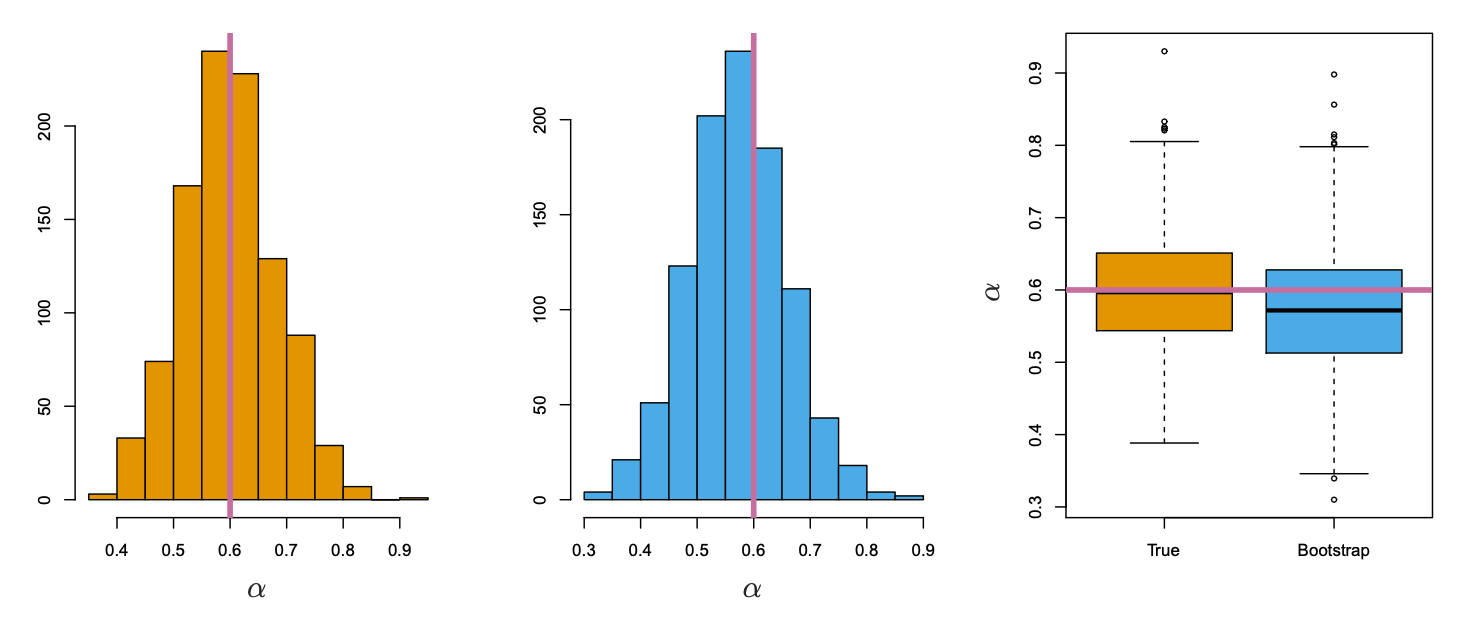
\includegraphics[width=10cm]{data/parameter.png}
            };
        \end{tikzpicture}
    }
\end{frame}

\begin{frame}{Model evaluation: Comparison}
    \only<1>{
        \textbf{Why do we want to evaluate our model?}
        \begin{enumerate}
            \item We want to show that our model is better than random guessing
            \item We want to show that our model is better than another model
        \end{enumerate}
    }
    \only<2-18>{
        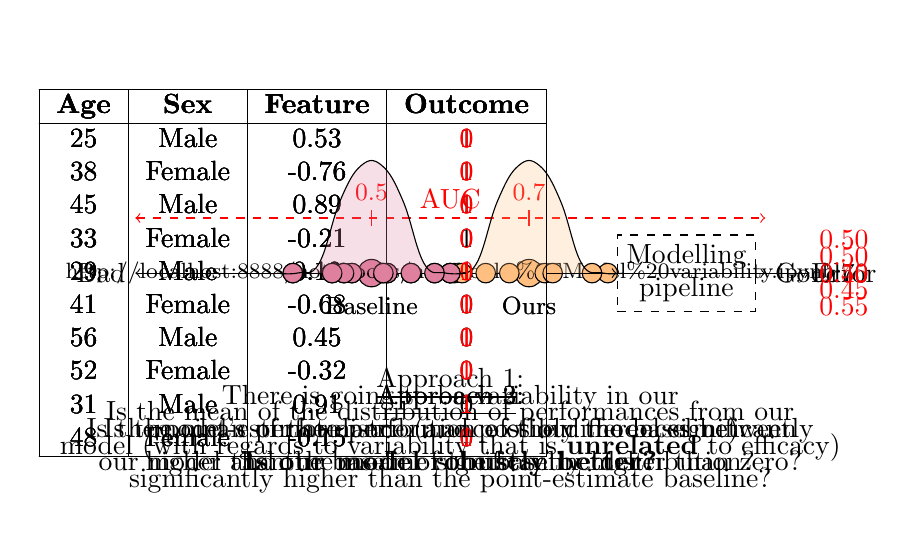
\begin{tikzpicture}
            \node[] at (-5, 3) {};
            \node[] at (5, -3) {};

            \visible<2-3,5-10,16-18>{
                \draw[<->] (-4, 0) -- (4, 0);
                \node[anchor=west] at (4, 0) {Good};
                \node[anchor=east] at (-4, 0) {Bad};
            }
            \visible<2-3,5-6,9-10,16-17>{
                \node[circle, inner sep=3.5pt, draw=black, fill=orange!50, label=below:\small{Ours}] at (1, 0) {};
            }
            \visible<7-8,18>{
                \node[anchor=north] at (1, -0.18) {\small{Ours}};
            }
            \visible<2-3,5-9>{
                \node[circle, inner sep=3.5pt, draw=black, fill=purple!50, label=below:\small{Baseline}] at (-1, 0) {};
            }
            \visible<10,16-18>{
                \node[anchor=north] at (-1, -0.18) {\small{Baseline}};
            }
            \visible<3>{
                \draw[<->, red, dashed] (-4, 0.7) -- (4, 0.7);
                \node[red, anchor=south] at (0, 0.7) {AUC};
                \draw[red] (1, 0.6) -- (1, 0.8);
                \draw[red] (-1, 0.6) -- (-1, 0.8);
                \node[font=\small, anchor=south, red] at (1, 0.8) {0.7};
                \node[font=\small, anchor=south, red] at (-1, 0.8) {0.5};
            }
            \visible<4>{
                \node[font=\footnotesize\selectfont, text width=10.5cm, align=center] at (0, 0) {
                    \url{http://localhost:8888/notebooks/notebooks\%2FModel\%20variability.ipynb}
                };
            }
            \visible<5>{
                \node[align=center] at (0, -2) {There is going to be variability in our\\model's performance (and possibly the baseline).\\ \textbf{Is our model robustly better?}};
            }
            \visible<6-8>{
                \node[align=center] at (0, -2) {\underline{Approach 1}:\\Is the mean of the distribution of performances from our\\model (with regards to variability that is \textbf{unrelated} to efficacy)\\significantly higher than the point-estimate baseline?};
            }
            \visible<7-8,18>{
                \node[circle, inner sep=2.5pt, draw=black, fill=orange!50] at (0, 0) {};
                \node[circle, inner sep=2.5pt, draw=black, fill=orange!50] at (2, 0) {};
                \node[circle, inner sep=2.5pt, draw=black, fill=orange!50] at (1.2, 0) {};
                \node[circle, inner sep=2.5pt, draw=black, fill=orange!50] at (0.75, 0) {};
                \node[circle, inner sep=2.5pt, draw=black, fill=orange!50] at (0.45, 0) {};
                \node[circle, inner sep=2.5pt, draw=black, fill=orange!50] at (1.3, 0) {};
                \node[circle, inner sep=2.5pt, draw=black, fill=orange!50] at (0.05, 0) {};
                \node[circle, inner sep=2.5pt, draw=black, fill=orange!50] at (0.15, 0) {};
                \node[circle, inner sep=2.5pt, draw=black, fill=orange!50] at (1.8, 0) {};
            }
            \visible<8,18>{
                \fill[orange!50, opacity=0.25] plot[smooth, tension=0.7] coordinates {(-0.2,0) (0.0667,0.002) (0.3334,0.124) (0.6,0.916) (0.8667,1.365) (1.1334,1.365) (1.4,0.916) (1.6667,0.124) (1.9334,0.002) (2.2,0)} -- (2.2,0) -- (-0.2,0) -- cycle;
                \draw plot[smooth, tension=0.7] coordinates {(-0.2,0) (0.0667,0.002) (0.3334,0.124) (0.6,0.916) (0.8667,1.365) (1.1334,1.365) (1.4,0.916) (1.6667,0.124) (1.9334,0.002) (2.2,0)};
            }
            \visible<9-10,16-17>{
                \node[align=center] at (0, -2) {\underline{Approach 2}:\\Is the point-estimate performance of our model significantly\\higher than the mean of the baseline distribution?};
            }
            \visible<10>{
                \node[circle, inner sep=2.5pt, draw=black, fill=purple!50] at (-2, 0) {};
                \node[circle, inner sep=2.5pt, draw=black, fill=purple!50] at (0, 0) {};
                \node[circle, inner sep=2.5pt, draw=black, fill=purple!50] at (-1.25, 0) {};
                \node[circle, inner sep=2.5pt, draw=black, fill=purple!50] at (-0.8, 0) {};
                \node[circle, inner sep=2.5pt, draw=black, fill=purple!50] at (-1.35, 0) {};
                \node[circle, inner sep=2.5pt, draw=black, fill=purple!50] at (-0.85, 0) {};
                \node[circle, inner sep=2.5pt, draw=black, fill=purple!50] at (-1.5, 0) {};
                \node[circle, inner sep=2.5pt, draw=black, fill=purple!50] at (-0.5, 0) {};
                \node[circle, inner sep=2.5pt, draw=black, fill=purple!50] at (-0.2, 0) {};
            }
            \visible<11-15>{
                \node[draw=black, dashed, align=center] (pipeline) at (3, 0) {Modelling\\pipeline};

                \visible<11>{
                    \node (error) at (5, 0) {Error};
                }
                \visible<11-12>{
                    \node[inner sep=0pt] (data) at (-2, 0) {
                        \begin{tabular}{|c|c|c|c|}
                            \hline
                            \textbf{Age}&\textbf{Sex}&\textbf{Feature}&\textbf{Outcome}\\
                            \hline
                            25 & Male   &  0.53 & 1 \\
                            38 & Female & -0.76 & 1 \\
                            45 & Male   &  0.89 & 1 \\
                            33 & Female & -0.21 & 1 \\
                            29 & Male   &  0.12 & 1 \\
                            41 & Female & -0.68 & 0 \\
                            56 & Male   &  0.45 & 0 \\
                            52 & Female & -0.32 & 0 \\
                            31 & Male   &  0.91 & 0 \\
                            48 & Female & -0.15 & 0 \\
                            \hline
                        \end{tabular}
                    };
                }
                \visible<12>{
                    \node (error) at (5, 0) {0.70};
                }
                \visible<13>{
                    \node[inner sep=0pt] (data) at (-2, 0) {
                        \begin{tabular}{|c|c|c|c|}
                            \hline
                            \textbf{Age}&\textbf{Sex}&\textbf{Feature}&\textbf{Outcome}\\
                            \hline
                            25 & Male   &  0.53 & \textcolor{red}{1} \\
                            38 & Female & -0.76 & \textcolor{red}{0} \\
                            45 & Male   &  0.89 & \textcolor{red}{1} \\
                            33 & Female & -0.21 & \textcolor{red}{0} \\
                            29 & Male   &  0.12 & \textcolor{red}{1} \\
                            41 & Female & -0.68 & \textcolor{red}{0} \\
                            56 & Male   &  0.45 & \textcolor{red}{1} \\
                            52 & Female & -0.32 & \textcolor{red}{0} \\
                            31 & Male   &  0.91 & \textcolor{red}{1} \\
                            48 & Female & -0.15 & \textcolor{red}{0} \\
                            \hline
                        \end{tabular}
                    };
                    \node (error) at (5, 0) {\textcolor{red}{0.50}};
                }
                \visible<14>{
                    \node[inner sep=0pt] (data) at (-2, 0) {
                        \begin{tabular}{|c|c|c|c|}
                            \hline
                            \textbf{Age}&\textbf{Sex}&\textbf{Feature}&\textbf{Outcome}\\
                            \hline
                            25 & Male   &  0.53 & \textcolor{red}{0} \\
                            38 & Female & -0.76 & \textcolor{red}{0} \\
                            45 & Male   &  0.89 & \textcolor{red}{0} \\
                            33 & Female & -0.21 & \textcolor{red}{0} \\
                            29 & Male   &  0.12 & \textcolor{red}{0} \\
                            41 & Female & -0.68 & \textcolor{red}{1} \\
                            56 & Male   &  0.45 & \textcolor{red}{1} \\
                            52 & Female & -0.32 & \textcolor{red}{1} \\
                            31 & Male   &  0.91 & \textcolor{red}{1} \\
                            48 & Female & -0.15 & \textcolor{red}{1} \\
                            \hline
                        \end{tabular}
                    };

                    \node[align=center] (error) at (5, 0) {\textcolor{red}{0.50} \\ \textcolor{red}{0.45}};
                }
                \visible<15>{
                    \node[inner sep=0pt] (data) at (-2, 0) {
                        \begin{tabular}{|c|c|c|c|}
                            \hline
                            \textbf{Age}&\textbf{Sex}&\textbf{Feature}&\textbf{Outcome}\\
                            \hline
                            25 & Male   &  0.53 & \textcolor{red}{0} \\
                            38 & Female & -0.76 & \textcolor{red}{1} \\
                            45 & Male   &  0.89 & \textcolor{red}{0} \\
                            33 & Female & -0.21 & \textcolor{red}{0} \\
                            29 & Male   &  0.12 & \textcolor{red}{1} \\
                            41 & Female & -0.68 & \textcolor{red}{1} \\
                            56 & Male   &  0.45 & \textcolor{red}{0} \\
                            52 & Female & -0.32 & \textcolor{red}{0} \\
                            31 & Male   &  0.91 & \textcolor{red}{1} \\
                            48 & Female & -0.15 & \textcolor{red}{1} \\
                            \hline
                        \end{tabular}
                    };

                    \node[align=center] (error) at (5, 0) {\textcolor{red}{0.50} \\ \textcolor{red}{0.45} \\ \textcolor{red}{0.55}};
                }

                \draw[->] (data) -- (pipeline);
                \draw[->] (pipeline) -- (error);
            }
            \visible<16-18>{
                \node[circle, inner sep=2.5pt, draw=black, fill=purple!50] at (-2, 0) {};
                \node[circle, inner sep=2.5pt, draw=black, fill=purple!50] at (0, 0) {};
                \node[circle, inner sep=2.5pt, draw=black, fill=purple!50] at (-1.25, 0) {};
                \node[circle, inner sep=2.5pt, draw=black, fill=purple!50] at (-0.8, 0) {};
                \node[circle, inner sep=2.5pt, draw=black, fill=purple!50] at (-1.35, 0) {};
                \node[circle, inner sep=2.5pt, draw=black, fill=purple!50] at (-0.85, 0) {};
                \node[circle, inner sep=2.5pt, draw=black, fill=purple!50] at (-1.5, 0) {};
                \node[circle, inner sep=2.5pt, draw=black, fill=purple!50] at (-0.5, 0) {};
                \node[circle, inner sep=2.5pt, draw=black, fill=purple!50] at (-0.2, 0) {};
            }
            \visible<17-18>{
                \fill[purple!50, opacity=0.25] plot[smooth, tension=0.7] coordinates {(-2.2,0) (-1.9333,0.002) (-1.6666,0.124) (-1.4,0.916) (-1.1333,1.365) (-0.8666,1.365) (-0.6,0.916) (-0.3333,0.124) (-0.0666,0.002) (0.2,0)} -- (2.2,0) -- (-0.2,0) -- cycle;
                \draw plot[smooth, tension=0.7] coordinates {(-2.2,0) (-1.9333,0.002) (-1.6666,0.124) (-1.4,0.916) (-1.1333,1.365) (-0.8666,1.365) (-0.6,0.916) (-0.3333,0.124) (-0.0666,0.002) (0.2,0)};
            }
            \visible<18>{
                \node[align=center, text width=10.5cm] at (0, -2) {\underline{Approach 3}:\\Is the mean of the distribution of the differences between our model and the baseline significantly higher than zero?};
            }
        \end{tikzpicture}
    }
\end{frame}

\begin{frame}{Model evaluation: Summary}
    \begin{itemize}
        {\small
            \item Model evaluation should \textbf{always} happen out-of-sample
            \item If n is big ($\geq 10000$), a train/validation split can be sufficient
            \item For smaller samples, k-fold cross-validation with $5 \leq k \leq 10$ is a good trade-off between bias and variance
            \item The bootstrap is an effective way of getting confidence intervals for model performance \textbf{and parameters}
            \item Cross-validation (or bootstrapping) will produce a distribution of model performances (although caution the correlation)
            \item Permutation testing can produce a distribution of baseline performances
        }
    \end{itemize}
\end{frame}